\documentclass{article}
\usepackage{amsmath}
\usepackage{graphicx}
\usepackage{fancyhdr}
\usepackage{array}
\usepackage{booktabs}
\usepackage[sorting=none]{biblatex}
\usepackage[margin=1in]{geometry}
\usepackage{listings}

\lstset{
    language=Python,                    % تنظیم زبان پایتون
    backgroundcolor=\color{white},      % رنگ پس‌زمینه سفید
    basicstyle=\ttfamily\footnotesize,  % استفاده از فونت monospaced
    keywordstyle=\color{blue},           % رنگ کلمات کلیدی
    commentstyle=\color{green},         % رنگ کامنت‌ها
    stringstyle=\color{red},            % رنگ رشته‌ها
    numbers=left,                       % شماره‌گذاری خطوط
    numberstyle=\tiny\color{gray},      % استایل شماره‌های خطوط
    stepnumber=1,                       % شماره‌گذاری هر خط
    numbersep=5pt,                      % فاصله شماره‌گذاری از کد
    showspaces=false,                   % نمایش فضاها
    showstringspaces=false,             % نمایش فضاها در رشته‌ها
    showtabs=false,                     % نمایش تب‌ها
    frame=single,                       % نمایش قاب دور کد
    rulecolor=\color{black},            % رنگ قاب دور کد
    tabsize=2,                          % اندازه تب‌ها
    captionpos=b,                       % عنوان در پایین قرار می‌گیرد
    breaklines=true,                    % تقسیم خط‌های طولانی
    breakatwhitespace=true              % تقسیم در فضای خالی
}
\usepackage[hidelinks]{hyperref}
\usepackage{subfigure}
\hypersetup{
    colorlinks=true,
    linkcolor=teal,
    filecolor=magenta,      
    urlcolor=teal,
    citecolor = teal
    }
\usepackage{xcolor}
\usepackage{xepersian}
\usepackage{fontspec}
\setlength\headheight{28pt} 
\addbibresource{bibliography.bib}
\settextfont[Scale=1.2]{IRLotus.TTF}
\setlatintextfont[Scale=1]{Times New Roman}
\renewcommand{\baselinestretch}{1.5}
\pagestyle{fancy}
\fancyhf{}
\rhead{
\includegraphics[width=1cm]{FaultD.png}مینی پروژه سوم درس یادگیری ماشین}
\lhead{\thepage}
\rfoot{امیر جهانگرد تکالو}
\lfoot{علیرضا امیری}
\renewcommand{\headrulewidth}{1pt}
\renewcommand{\footrulewidth}{1pt}
\AtBeginDocument{
	\def\chapterautorefname{فصل}%
	\def\sectionautorefname{پاسخ سوال}%
	\def\subsectionautorefname{بخش}%
	\def\subsubsectionautorefname{بخش}%
	\def\equationautorefname{رابطهٔ}%
    \def\lstlistingautorefname{برنامۀ}%
}
\renewcommand{\lstlistingname}{Code}
\begin{document}

\input{titlepage}


\tableofcontents
\newpage


\section{1.SVM}

برای مشاهده نوت‌بوک من اینجا کلیک کنید:
 \href{https://drive.google.com/file/d/1nfyxbJQEZa4AznaHtXdWtNYiyUrZ2R4M/view?usp=sharing}{لینک گوگل کولب}
 
\subsection{1.1}

در این بخش به توضیح فرایند حل یک مسئله ی SVM با قید سخت (Hard Margin) خواهیم پرداخت.
به طور کلی، این مسئله به صورت یک فرایند بهینه سازی به شرح زیر تعریف می شود:

\begin{align*}
\min_{\mathbf{w}, b} \quad &amp; \frac{1}{2} \|\mathbf{w}\|^2 \\
\text{subject to} \quad &amp; y_i(\mathbf{w}^\top \mathbf{x}_i + b) \geq 1 \quad \forall i
\end{align*}


که در آن، w بردار های وزن، b  مقادیر بایاس، y برچسب ها و x بردار ورودی است.

برای یافتن مقدار بهینه ی این سوال، از دوگان روابط بالا استفاده می شود و به جای حل مسئله ی کمینه سازی، این مسئله را به صورت بیشینه سازی به صورت زیر تعریف می کنیم. 
    \begin{align*}
\max_{\boldsymbol{\alpha}} \quad &amp; \sum_{i=1}^n \alpha_i - \frac{1}{2} \sum_{i,j=1}^n \alpha_i \alpha_j y_i y_j \mathbf{x}_i^\top \mathbf{x}_j \\
\text{subject to} \quad &amp; \sum_{i=1}^n \alpha_i y_i = 0, \\
&amp; \alpha_i \geq 0 \quad \forall i
\end{align*}

حال برای استفاده در کد بهینه سازی و تبدیل این معادلات به فرمت ماتریسی، در نهایت خواهیم داشت:
    \begin{align*}
\min_{\boldsymbol{\alpha}} \quad &amp; \frac{1}{2} \boldsymbol{\alpha}^\top P \boldsymbol{\alpha} + \mathbf{q}^\top \boldsymbol{\alpha} \\
\text{subject to} \quad &amp; G \boldsymbol{\alpha} \leq \mathbf{h}, \\
&amp; A \boldsymbol{\alpha} = b
\end{align*}

که در آن:
\[
\begin{aligned}
P &= (y_i y_j)(\mathbf{x}_i^\top \mathbf{x}_j) \\
\mathbf{q} &= -\mathbf{1} \\
G &= -I \\
\mathbf{h} &= \mathbf{0} \\
A &= y^\top \\
b &= 0
\end{aligned}
\]
در شکل \autoref{fig:1} صفحه ی به دست آمده برای این مسئله نمایش داده شده است.

\begin{figure}[h!]
    \centering
    
\includegraphics[width=0.75\linewidth]{1.png}
    \caption{نمایش svm}
    \label{fig:1}
\end{figure}

که در آن پارامتر های صفحه به صورت زیر خواهند بود:
\[
\mathbf{w} = \begin{bmatrix}
-0.499956384 \\
-0.000174464249 \\
1.0
\end{bmatrix}, \quad
b = -1.4998865982379106
\]
\subsection{1.2}
\subsubsection{1.2.1}
در این بخش، دیتاست معیار آلودگی هوای پکن را دانلود کرده و پس از ذخیره ی آ« به عنوان یک دیتافریم، پند سطر ابتدای آن را مشاهده می کنیم.
\begin{figure}[h!]
    \centering
    
\includegraphics[width=0.75\linewidth]{2.png}
    \caption{سطر های اول دیتاست خام}
    \label{fig:2}
\end{figure}
\clearpage

با بررسی ویژگی های موجود در این دیتافریم به شرح زیر خواهیم داشت:
\begin{table}[h!]
\centering
\begin{tabular}{| l | l | p{9cm} |}
\hline
\textbf{Feature} & \textbf{Type} & \textbf{Description} \\
\hline
\textbf{No}     & Integer     & Row index (not necessary for modeling) \\
\textbf{year}   & Integer     & Year of observation (2010 to 2014) \\
\textbf{month}  & Integer     & Month (1–12) \\
\textbf{day}    & Integer     & Day of the month (1–31) \\
\textbf{hour}   & Integer     & Hour of the day (0–23) \\
\textbf{pm2.5}  & Float       & PM2.5 concentration in micrograms/m\textsuperscript{3} (target variable for pollution) \\
\textbf{DEWP}   & Float       & Dew Point (°C) \\
\textbf{TEMP}   & Float       & Temperature (°C) \\
\textbf{PRES}   & Float       & Atmospheric pressure (hPa) \\
\textbf{cbwd}   & Categorical & Combined wind direction (e.g., 'NW', 'NE', 'SE', 'cv') \\
\textbf{Iws}    & Float       & Cumulated wind speed (m/s) \\
\textbf{Is}     & Float       & Cumulated hours of snow \\
\textbf{Ir}     & Float       & Cumulated hours of rain \\
\hline
\end{tabular}
\caption{Description of features in the PM2.5 dataset}
\end{table}

با این ویژگی ها؛ مشاهده می کنیم که مقدار pm2.5 به طور مشخص معیار اندازه گیری شده از آلودگی هوا است و در این پژوهش، به عنوان هدف در نظر گرفته می شود. 
به غیر از این ستون، ویژگی های زمانی مانند سال و ماه و روز، یا ویژگی های جوی مانند فشار، دمای شبنمی و دمای هوا، ویژگی های مربوط بهخ رطوبت هوا از جمله باران و برف، و ویژگی هیا مربوط به جهت باد هر یک می توانند تاثیر به سزایی در تشخیص آلودگی داشته باشند.
\subsubsection{1.2.2}

در اینجا، به بررسی ساختار و داده های موجود در دیتافریم حاضر خواهیم پرداخت. 
ابتدا وجود داده های NaN را بررسی می کنیم. همان طور که در \autoref{fig:3} مشاهده می شود، تنها مقادیر هدف برای تعدادی از داده ها مجهول هستند که در ادامه باید رفع شوند.
]{}
\begin{figure}[h!]
    \centering
    
\includegraphics[width=0.75\linewidth]{3.png}
    \caption{بررسی داده های Nan}
    \label{fig:3}
\end{figure}

حال به بررسی توزیع داده ها خواهیم پرداخت.
\begin{figure}[h!]
    \centering
    
\includegraphics[width=0.75\linewidth]{4.png}
    \caption{توزیع داده های عددی دیتافریم}
    \label{fig:4}
\end{figure}

\begin{figure}[h!]
    \centering
    
\includegraphics[width=0.75\linewidth]{5.png}
    \caption{توزیع داده های دسته بندی دیتافریم}
    \label{fig:5}
\end{figure}

و برای بررسی داده همبستگی داده ها، ماتریس همبستگی را رسم می کنیم.
\begin{figure}[h!]
    \centering
    
\includegraphics[width=0.75\linewidth]{6.png}
    \caption{ماتریس همبستگی}
    \label{fig:6}
\end{figure}

می توان نتیجه گرفت که دیتافریم موجود دارای ستون هایی برای مقادیر زمانی است که به طور مستقیم ویژگی نیستند و باید از آنها ویژگی استخراج شود. 
علاوه بر این، توزیع داده های pm2.5 نشان می دهد که بیشتر داده ها در سمت آلودگی کمتر قرار دارند ام ا طولانی بودن انتهای این توزیع نشان دهنده ی وجود مقادیری با آلودگی های زیاد نیز هست. که این نشان دهنده ی نیاز به تقسیم بازه های این ویژگی و binning است. علاوه بر این، در نظر گرفتن outlier ها در اینجا اهمیت پیدا می کند.

\subsubsection{1.2.3}
حال در اینجا به کنترل وضعیت داده های NaN خواهیم پرداخت. چنان که بیان شد، تنها تعدادی از داده های pm2.5 مجهول هستند و از آنجا که این مقادیر خود هدف مسئله هستند، نمی توان برای آنها داده هایی را درون یابی کرد، چرا که این امر به معنی وارد کردن داده های نامطمئن به دیتاست خواهد بود. 
با این حال، از آنجا که داده ها در این دیتافریم وابستگی زمانی دارند و در ادامه ی فرایند لازم است از داده های گذشته برای تعیین ویژگی های داده های آینده استفاده شود، حذف این سطر ها در ادامه به بروز مشکلاتی منجر می شود. 
بنابراین، با در نظر داشتن این مورد که در نهایت این سطر ها باید حذف شوند، فعلا آنها را نگه می داریم تا ابتدا فرایند استخراج ویژگی های زمانی انجام شود و سپس این داده ها را حذف می کنیم.

در اینجا، ویژگی های زمانی مربوط به مقادیر گذشته ی pm2.5 در 1،2،3،24 و 168 ساعت گذشته را برای هر داده به دست می آوریم.
پس از استخارج این ویژگی ها، می توانیم سطر هایی که مقادیر گذشته ی آنها وجود ندارد و همچنین سطر هایی که مقدار هدف آنها NAN است را حذف کنیم.
\begin{figure}[h!]
    \centering
    
\includegraphics[width=0.5\linewidth]{7.png}
    \caption{7}
    \label{fig:7}
\end{figure}

\begin{figure}[h!]
    \centering
    
\includegraphics[width=0.5\linewidth]{8.png}
    \caption{میزان داده های NaN}
    \label{fig:8}
\end{figure}

\subsubsection{1.2.4}
در این بخش، به بررسی داده های دسته بندی خواهیم پرداخت. مشاهده می کتیم که تنها  ستون با این نوع داده، مربوط به جهت باد است که دسته بندی های آن در \autoref{fig:5} نمایش داده شده است.
برای تبدیل این داده های این ستون به مقادیر عددی، از روش $One Hot Encoding$ استفاده شده است و در نتجه، چهار ستون به جای آن تعریف می شود.\autoref{}
\begin{figure}[h!]
    \centering
    
\includegraphics[width=0.5\linewidth]{9.png}
    \caption{One hot encoding}
    \label{fig:9}
\end{figure}

\subsubsection{1.2.5}
در این بخش به بررسی داده های پرت خواهیم پرداخت.
می دانیم که وجود این مقادیر در دیاست، می تواند مدل را به دلیل وجود تعداد کمی داده ی پرت، از یادگیری بخش غالب داده ها منحرف کند. این مقادیر به دلیل آنکه مقدار بسیار بیشتر و یا کمتری دارند، تاثیر بیشتری بر وزن های سیستم خواهند داشت و در نتیجه بسیار مهم است که بتوانیم آنها را مدیریت کنیم. برای این منظور، در دیتاست حاضر، توزیع ویژگی هایی که مقادیر عددی دارند را به صورت boxPlot رسم  می کنیم
\begin{figure}[h!]
    \centering
    
\includegraphics[width=0.75\linewidth]{10.png}
    \caption{توزیع ویژگی های عددی برای پیدا کردن دادده های پرت}
    \label{fig:10}
\end{figure}

همان طور که مشاهده می شود، در ستون های lws و pm2.5 داده های پرت وجود دارد. 
مجددا با توجه به اینکه داده های موجود در pm2.5 مقادیر هدف هستند، نمی توان آنها را تغییر داد و یا حذف کرد. 
اما برای ستون lws، ابتدا توزیع آن را مشاهده می کنیم.
\begin{figure}[h!]
    \centering
    
\includegraphics[width=0.75\linewidth]{11.png}
    \caption{توزیع داده های lws}
    \label{fig:11}
\end{figure}

در \autoref{fig:11} توزیع داده های lws را مشاهده می کنیم.
برای رفع مشکل داده های پرت در این ستون، از روش capping استفاده می کنیم. به هاین صورت که مقادیر بیشتر  از 99 درصد داده ها برابر با بیشترین داده در این بازه و و مقادیر کمتر از 1 درصد داده ها برابر با کمترین داده در این بازه تعیین می شود.

در نتیجه، توزیع داده ها پس از اعمال این تغییرات به صورت زیر خواهد بود.
\begin{figure}[h!]
    \centering
    
\includegraphics[width=0.75\linewidth]{12.png}
    \caption{توزیع داده ها پس از حدف داده های پرت}
    \label{fig:12}
\end{figure}

\subsubsection{1.2.6}
هدف از پیاده سازی این بخش، تقسیم داده ها به مقادیر دسته بندی به جای مقادیر عددی است. برای این منظور، مطابق جدول زیر داده ها را تقسیم می کنیم.
\begin{table}[h!]
\centering
\begin{tabular}{|l|c|}
\hline
\textbf{AQI Category} & \textbf{PM2.5 Range (µg/m\textsuperscript{3})} \\
\hline
Good                           & 0.0 -- 12.0 \\
Moderate                       & 12.1 -- 35.4 \\
Unhealthy for Sensitive Groups & 35.5 -- 55.4 \\
Unhealthy                      & 55.5 -- 150.4 \\
Very Unhealthy                 & 150.5 -- 250.4 \\
Hazardous                      & 250.5 -- 500 \\
Extreme                        & > 500 \\
\hline
\end{tabular}
\caption{AQI Categories Based on PM2.5 Concentration}
\end{table}
پس از این تقسیم، توزیع داده ها به صورت زیر به دست خواهد آمد.
\begin{figure}[h!]
    \centering
    
\includegraphics[width=0.75\linewidth]{13.png}
    \caption{توزیع داده ها پس از دسته بندی مقدار هدف}
    \label{fig:13}
\end{figure}
\begin{figure}[h!]
    \centering
    
\includegraphics[width=0.75\linewidth]{14.png}
    \caption{نمودار پای توزیع داده ها}
    \label{fig:14}
\end{figure}

\subsubsection{1.2.7}
مطابق با خواسته ی سوال، در این بخش لازم است ویژگی های Lag بر اساس داده های قبلی استخراج شوند. اما به دلیل آنکه قصد داشتیم داده های NaN را حذف کنیم، پیش از این این موارد را اضافه کنیم. 
در اختیار داشتن داده های قبلی، می تواند اطلاعاتی از روند تغییرات را به مدل آموزش دهد و معیار تصمیم گیری آن را نه تنها بر اساس داده های فعلی، که بر اساس داده های قبلی تعیین کند.
با این حال، در داده های ابتدایی که به این تعداد از داده های قبل در اختیار نداریم، مقادیر NAN باقی خواهد ماند. 
به دلیل آنکه به این تعداد از داده های قبل را در اختیار نداریم، نمی توانیم این داده ها را نگه داریم و ناچار به حذف آن خواهیم بود.

حال به رسم نمودار این داده های با تاخیر خواهیم پرداخت.\autoref{fig:15}
\begin{figure}[h!]
    \centering
    
\includegraphics[width=1\linewidth]{15.png}
    \caption{نمودار تغییرات آلودگی هوا با معیار های تاخیردار}
    \label{fig:15}
\end{figure}

سپس، میزان همبستگی این مقادیر را با مقدار لحظه ای رسم می کنیم.
\begin{figure}[h!]
    \centering
    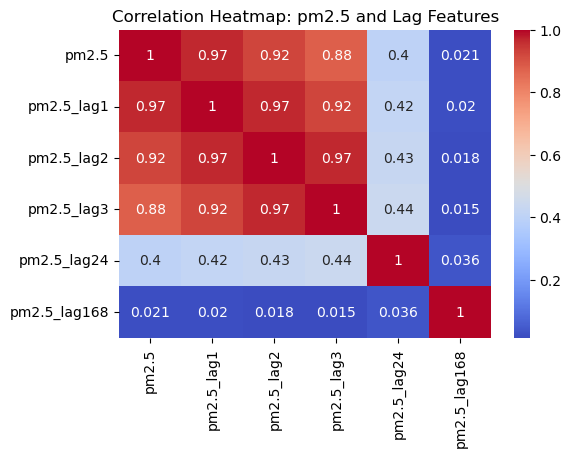
\includegraphics[width=0.53\linewidth]{16.png}
    \caption{همبستگی ویژگی های زمانی}
    \label{fig:16}
\end{figure}
چنان که انتظار می رود، همبستگی این داده ها با داده های نزدیک بسیار بیشتر است و روند آن با داده های قدیمی تر کمتر می شود.

حال به ایجاد ویژگی های Rolling و آماری بر روی داده ها خواهیم پرداخت.
این ویژگی ها به صورت زیر خواهند بود و بر اساس داده های 24 ساعت گذشته تعریف می شوند.
\begin{itemize}
  \item \texttt{pm2.5\_roll\_mean\_24h} -- 24-hour rolling mean of PM2.5
  \item \texttt{pm2.5\_roll\_std\_24h} -- 24-hour rolling standard deviation of PM2.5
  \item \texttt{pm2.5\_roll\_var\_24h} -- 24-hour rolling variance of PM2.5
  \item \texttt{pm2.5\_roll\_min\_24h} -- 24-hour rolling minimum of PM2.5
  \item \texttt{pm2.5\_roll\_max\_24h} -- 24-hour rolling maximum of PM2.5
  \item \texttt{pm2.5\_roll\_median\_24h} -- 24-hour rolling median of PM2.5
  \item \texttt{pm2.5\_roll\_skew\_24h} -- 24-hour rolling skewness of PM2.5
  \item \texttt{pm2.5\_roll\_kurt\_24h} -- 24-hour rolling kurtosis of PM2.5
\end{itemize}

به طور طبیعی اگر بخواهیم این فرایند را برای تمام داده ها لحاظ کنیم، در مقادیر اول یا مقدار NAN خواهیم داشت و یا مقادیر ثابت می شوند. اما برای این داده ها در صورتی که پنجره زمانی را انعطاف پذیر در نظر بگیریم و تنها ویژگی های مربوط به داده های قبلی آن را در محاسبه لحاظ کنیم، آنگاه مقادیر ثابت یا NAN باقی نمی ماند.
\begin{figure}[h!]
    \centering
    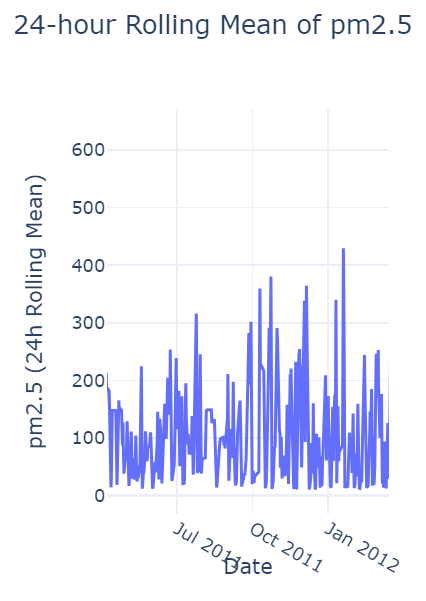
\includegraphics[width=0.53\linewidth]{17.png}
    \caption{نمودار میانگین 24 ساعت گذشته}
    \label{fig:17}
\end{figure}
\newpage
در گام بعد، به انکود کردن ویژگی های تناوبی خواهیم پرداخت. 
از آنجا که در این دیتافریم معیارهای زمانی مانند ساعت، روز، هفته، ماه و فصل و سال وجود دارد، و اتفاقات موجود به صورت تکرار شونده در این بازه ها رخ می دهند، بنابراین در نظر داشتن این تناوب اهمیت زیادی خواهد داشت.

با استفاده از تبدیل فوریه، مقادیر تناوبی را به دست می آوریم.
\begin{figure}[h!]
    \centering
    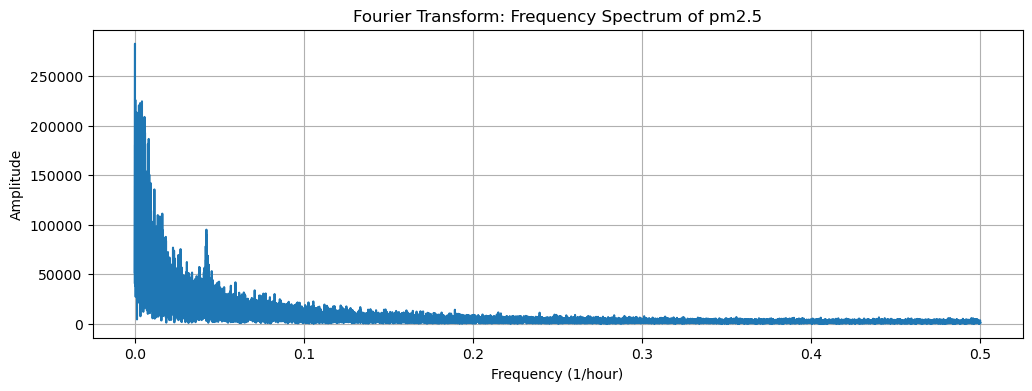
\includegraphics[width=0.75\linewidth]{18.png}
    \caption{فرکانس های غالب داده ها}
    \label{fig:18}
\end{figure}

\begin{figure}[h!]
    \centering
    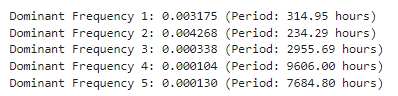
\includegraphics[width=0.75\linewidth]{19.png}
    \caption{دامنه ها}
    \label{fig:19}
\end{figure}


کد ارائه‌شده از \textbf{تبدیل فوریه (FFT)} برای تحلیل طیف فرکانسی داده‌های PM2.5 استفاده کرده است. در مرحله اول، مقادیر PM2.5 از دیتاست استخراج و مقادیر گمشده (\texttt{NaN}) حذف شده‌اند. سپس با استفاده از تابع \texttt{fft} از کتابخانه \texttt{scipy}، طیف فرکانسی محاسبه شده و تنها فرکانس‌های مثبت برای تحلیل حفظ شده‌اند. در نهایت، نمودار دامنه برحسب فرکانس (با واحد 1/hour) رسم شده و 5 فرکانس غالب با بیشترین دامنه شناسایی شده‌اند. اگرچه این کد مستقیماً به انکودینگ ویژگی‌های تناوبی نپرداخته، اما نتایج آن می‌تواند برای شناسایی الگوهای زمانی تکرارشونده در داده‌های PM2.5 مفید باشد.


نتایج تحلیل FFT نشان می‌دهد که بالاترین دامنه مربوط به فرکانس 0.003175 \lr{(1/hour)} با دوره تناوب 314.95 ساعت (~13 روز) است که احتمالاً نشان‌دهنده الگوی فصلی در آلودگی هوا می‌باشد. نمودار طیف فرکانسی تأیید می‌کند که بیشترین انرژی سیگنال در فرکانس‌های پایین متمرکز است، که نشان‌دهنده تغییرات بلندمدت در داده‌های PM2.5 است. این یافته‌ها می‌توانند به طراحی ویژگی‌های تناوبی هوشمند برای بهبود مدل‌های پیش‌بینی کمک کنند، هرچند برای نتیجه‌گیری دقیق‌تر نیاز به بررسی بیشتر وجود دارد.

در ادامه کد ارائه‌شده یک هیت‌مپ (نقشه حرارتی) برای نمایش میانگین غلظت ذرات PM2.5 بر اساس ساعات روز و ماه‌های سال ایجاد کرده است. در این کد، ابتدا با استفاده از تابع \texttt{groupby}، داده‌ها بر اساس ماه و ساعت گروه‌بندی شده و میانگین PM2.5 برای هر ترکیب ماه-ساعت محاسبه شده است. سپس با استفاده از کتابخانه \texttt{seaborn} و تابع \texttt{heatmap}، این داده‌ها به صورت یک ماتریس دو بعدی با رنگ‌بندی \texttt{coolwarm} نمایش داده شده‌اند. محور افقی نشان‌دهنده ساعات روز (0 تا 23) و محور عمودی نشان‌دهنده ماه‌های سال (1 تا 12) می‌باشد.

\begin{figure}[h!]
    \centering
    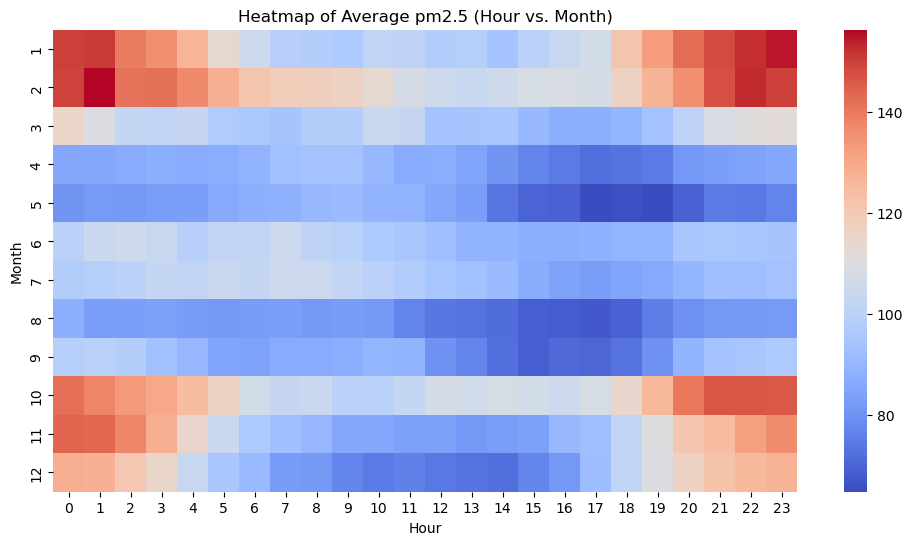
\includegraphics[width=0.75\linewidth]{20.png}
    \caption{نمودار هیت مپ}
    \label{fig:20}
\end{figure}

نتایج هیت‌مپ نشان می‌دهد که الگوی تغییرات PM2.5 هم به ساعت روز و هم به ماه سال وابسته است. بیشترین غلظت آلودگی در ساعات صبح (معمولاً بین ساعت 8 تا 10) و همچنین در ماه‌های سرد سال مشاهده می‌شود که احتمالاً به دلیل وارونگی دمایی و افزایش فعالیت‌های انسانی است. در مقابل، کمترین میزان آلودگی در ساعات اولیه صبح (4 تا 6) و ماه‌های گرمتر دیده می‌شود. این الگوها می‌توانند برای پیش‌بینی بهتر آلودگی هوا و برنامه‌ریزی راهکارهای کاهش آن مورد استفاده قرار گیرند.



در ادامه پروژه، برای بررسی الگوی تغییرات آلودگی هوا، میانگین غلظت ذرات PM2.5 بر اساس ساعات روز و سال‌های مختلف محاسبه شده است. در این بخش، داده‌ها ابتدا بر اساس سال و ساعت گروه‌بندی گردیدند و سپس با استفاده از تکنیک نقشه حرارتی، نتایج به صورت گرافیکی نمایش داده شدند. این روش امکان شناسایی الگوهای زمانی را به خوبی فراهم می‌کند، به طوری که محور افقی نشان‌دهنده ساعات شبانه‌روز و محور عمودی سال‌های مورد مطالعه را نمایش می‌دهد.

\begin{figure}[h!]
    \centering
    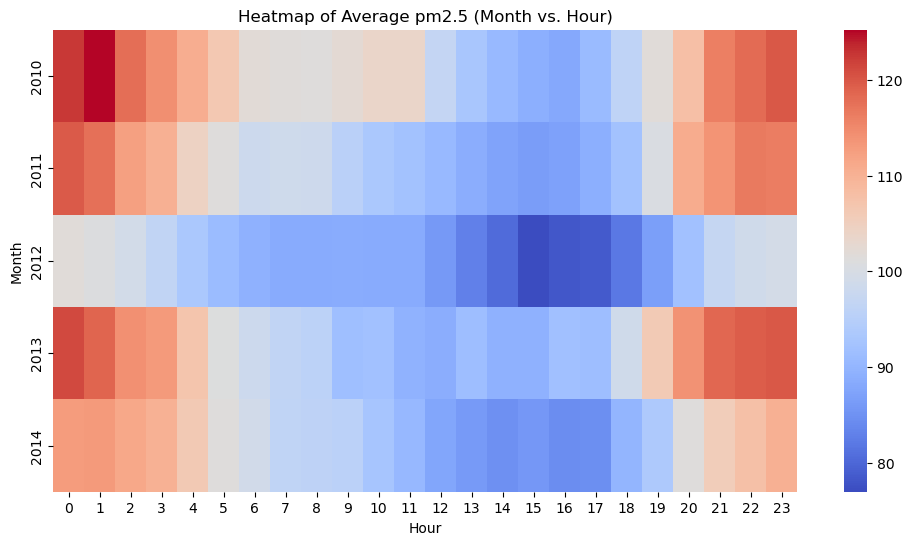
\includegraphics[width=0.75\linewidth]{21.png}
    \caption{نمودار هیت مپ ساعت به سال}
    \label{fig:21}
\end{figure}

نتایج حاصل از این تحلیل نشان می‌دهد که توزیع آلودگی هوا در ساعات مختلف روز و سال‌های متفاوت، تغییرات قابل توجهی دارد. در اینجا مشاهده می‌شود که بیشترین غلظت ذرات معلق معمولاً در ساعات میانی روز و همچنین در سال‌های خاصی رخ می‌دهد. این الگوها احتمالاً به عوامل مختلفی از جمله تغییرات آب‌وهوایی، فعالیت‌های انسانی و سیاست‌های محیط زیستی مرتبط هستند. سپس با مقایسه سال‌های مختلف می‌توان روند تغییرات آلودگی هوا را در طول زمان بررسی کرد که برای برنامه‌ریزی‌های آینده بسیار ارزشمند خواهد بود.



در این مرحله از پروژه، به بررسی تغییرات غلظت ذرات PM2.5 در طول هفته پرداخته شده است. ابتدا با استخراج روزهای هفته از داده‌های زمانی، میانگین آلودگی برای هر ساعت از روزهای مختلف محاسبه گردید. سپس این اطلاعات به صورت یک نقشه حرارتی سازماندهی شد که در آن محور عمودی نشان‌دهنده روزهای هفته (از دوشنبه تا جمعه) و محور افقی ساعات شبانه‌روز را نمایش می‌دهد. این رویکرد امکان شناسایی الگوهای هفتگی آلودگی هوا را فراهم می‌سازد.

\begin{figure}[h!]
    \centering
    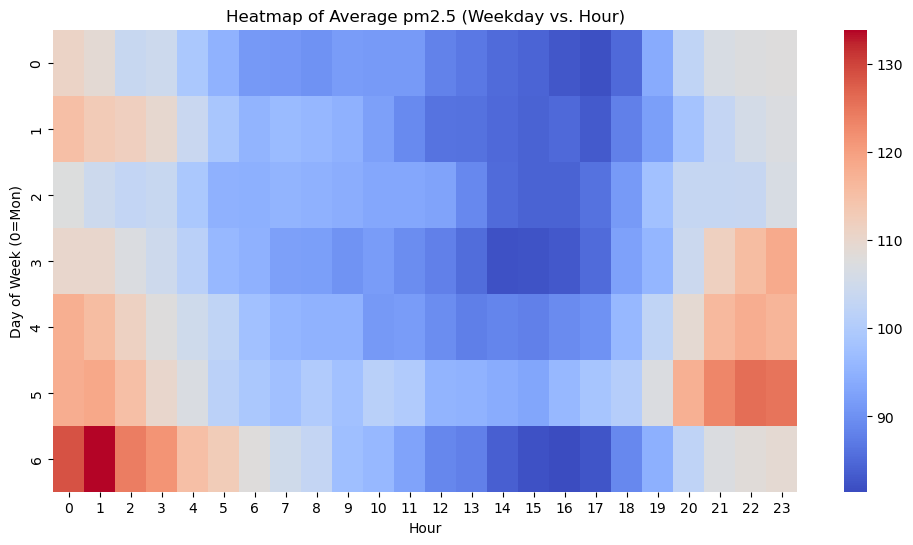
\includegraphics[width=0.75\linewidth]{22.png}
    \caption{نمودار هیت مپ}
    \label{fig:22}
\end{figure}

نتایج این تحلیل الگوی جالبی از تغییرات آلودگی هوا را نشان می‌دهد. به طور مشخص، روزهای میانی هفته (سه‌شنبه تا پنجشنبه) در ساعات اوج ترافیک صبحگاهی و عصرگاهی، بالاترین غلظت PM2.5 را دارند. همچنین مشاهده می‌شود که روزهای پایانی هفته (جمعه) الگوی متفاوتی را نمایش می‌دهند که احتمالاً به دلیل کاهش فعالیت‌های صنعتی و ترافیکی است. این یافته‌ها می‌توانند برای برنامه‌ریزی‌های شهری و مدیریت ترافیک در روزهای مختلف هفته مورد استفاده قرار گیرند.


در ادامه بررسی الگوهای زمانی آلودگی هوا، از روش کدگذاری چرخه‌ای برای ویژگی‌های زمانی شامل ساعت روز، روز هفته و ماه سال استفاده شد. این روش با اعمال توابع سینوسی و کسینوسی بر روی مقادیر زمانی، ماهیت چرخشی آنها را حفظ می‌کند. سپس برای نمایش گرافیکی، میانگین غلظت PM2.5 در ساعات مختلف روز بر روی یک نمودار دایره‌ای با تقسیم‌بندی دوره‌های زمانی مختلف (شب، سحرگاه، روز و غروب) ترسیم شد. هر نقطه در این نمودار نشان‌دهنده یک ساعت خاص از روز است که رنگ آن بیانگر میزان آلودگی در آن ساعت می‌باشد.

\begin{figure}[h!]
    \centering
    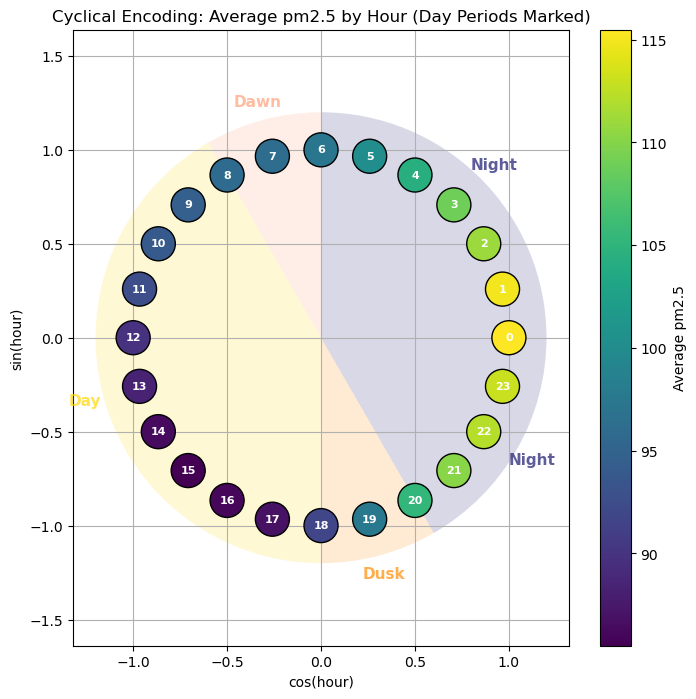
\includegraphics[width=0.75\linewidth]{23.png}
    \caption{نمودار انکودینگ چرخه ای در ساعت}
    \label{fig:23}
\end{figure}

نتایج این تحلیل الگوی جالبی از تغییرات آلودگی هوا در طول روز را نشان می‌دهد. بیشترین غلظت ذرات معلق در ساعات روز (بین 8 تا 17) مشاهده می‌شود که همزمان با اوج فعالیت‌های انسانی و ترافیک شهری است. در مقابل، کمترین میزان آلودگی در ساعات شب (20 تا 5 صبح) ثبت شده است. نکته قابل توجه تفاوت محسوس بین ساعات سحرگاه و غروب است که احتمالاً به عوامل جوی و تغییرات دمایی مربوط می‌شود. این یافته‌ها می‌تواند در برنامه‌ریزی‌های شهری و مدیریت ترافیک مورد استفاده قرار گیرد.

\newpage
در این بخش از تحلیل، الگوی تغییرات فصلی غلظت ذرات PM2.5 با استفاده از روش کدگذاری چرخه‌ای ماهانه مورد بررسی قرار گرفته است. ابتدا میانگین ماهانه آلودگی هوا محاسبه شده و سپس با اعمال تبدیلات سینوسی و کسینوسی، ماهیت چرخشی فصول حفظ گردیده است. برای نمایش بصری، یک نمودار دایره‌ای طراحی شده که در آن هر نقطه نشان‌دهنده یک ماه خاص بوده و رنگ آن بیانگر میزان متوسط آلودگی در آن ماه می‌باشد. همچنین مناطق مختلف نمودار با رنگ‌های متمایز برای فصول چهارگانه سال (زمستان، بهار، تابستان و پاییز) مشخص شده‌اند.

\begin{figure}[h!]
    \centering
    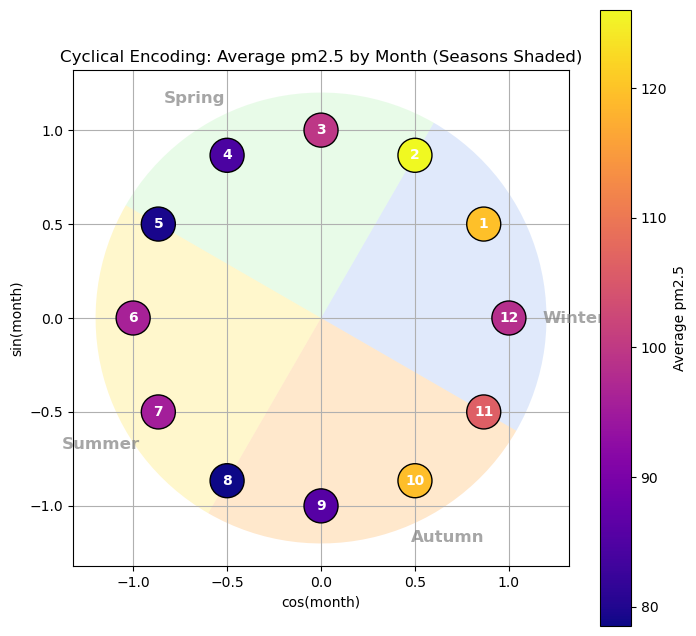
\includegraphics[width=0.75\linewidth]{24.png}
    \caption{نمودار انکودینگ چرخه ای در ماه}
    \label{fig:24}
\end{figure}


نتایج این تحلیل نشان می‌دهد که الگوی تغییرات آلودگی هوا از توزیع فصلی مشخصی پیروی می‌کند. بیشترین غلظت ذرات معلق در ماه‌های زمستان (دی، بهمن و اسفند) مشاهده می‌شود که احتمالاً ناشی از پدیده وارونگی دمایی و افزایش مصرف سوخت‌های فسیلی است. در مقابل، کمترین میزان آلودگی در ماه‌های تابستان (خرداد تا شهریور) ثبت شده که با بهبود شرایط جوی و کاهش پایداری هوا مرتبط می‌باشد. نکته جالب توجه، کاهش تدریجی آلودگی از فصل پاییز به زمستان و سپس افزایش ناگهانی آن در اواسط زمستان است که می‌تواند نشان‌دهنده تأثیر همزمان عوامل جوی و انسانی باشد.

\newpage
در این بخش از پژوهش، الگوی هفتگی تغییرات آلودگی هوا با استفاده از کدگذاری چرخه‌ای روزهای هفته مورد بررسی قرار گرفته است. ابتدا میانگین غلظت PM2.5 برای هر روز هفته محاسبه شده و سپس با تبدیل سینوسی-کسینوسی، ماهیت تناوبی هفته حفظ گردیده است. نمودار دایره‌ای طراحی شده، روزهای هفته را به چهار بخش «تعطیل»، «ابتدای هفته»، «میانه هفته» و «پایان هفته» تقسیم کرده که هر بخش با رنگ متمایزی مشخص شده است. هر نقطه در این نمودار نمایانگر یک روز خاص بوده و رنگ آن بیانگر میزان متوسط آلودگی در آن روز می‌باشد.

\begin{figure}[h!]
    \centering
    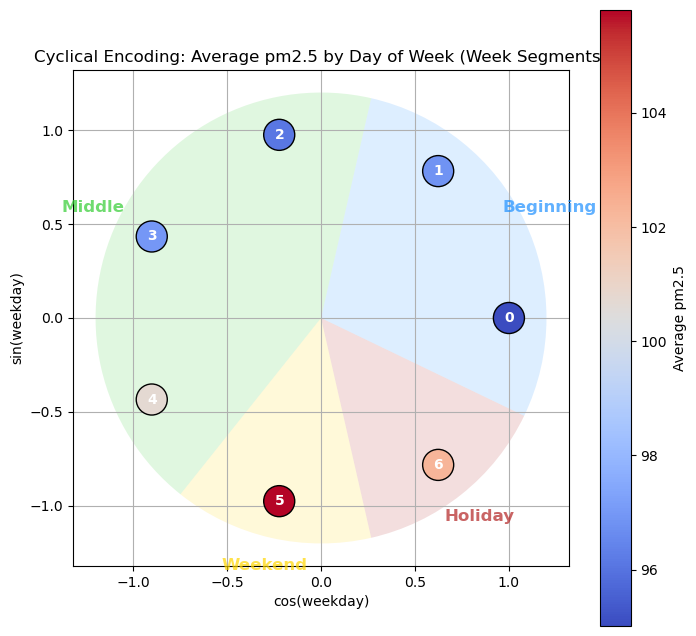
\includegraphics[width=0.75\linewidth]{25.png}
    \caption{نمودار انکودینگ چرخه ای در هفته}
    \label{fig:25}
\end{figure}


نتایج تحلیل نشان می‌دهد که الگوی آلودگی هوا در طول هفته نوسانات معناداری دارد. بیشترین غلظت ذرات معلق در روزهای میانی هفته (سه‌شنبه تا پنجشنبه) مشاهده می‌شود که احتمالاً ناشی از فعالیت‌های صنعتی و ترافیک کاری است. در مقابل، روزهای تعطیل (یکشنبه) کمترین میزان آلودگی را نشان می‌دهند. نکته جالب توجه، کاهش محسوس آلودگی در روزهای پایانی هفته (جمعه) نسبت به روزهای میانی است که می‌تواند نشان‌دهنده کاهش فعالیت‌های اقتصادی در آستانه تعطیلات باشد. این یافته‌ها برای برنامه‌ریزی‌های مدیریت ترافیک و کنترل آلودگی هوا در روزهای مختلف هفته حائز اهمیت است.

\newpage

به طور خلاصه در این دیتاست، ویژگی‌های تناوبی متعددی شامل ساعت روز، روز هفته و ماه سال وجود دارد که به دلیل ماهیت چرخشی‌شان نیاز به کدگذاری ویژه دارند. برای انکودینگ این ویژگی‌ها از روش سینوسی-کسینوسی استفاده شده است، چرا که این روش با تبدیل مقادیر خطی به مختصات دایره‌ای، فاصله‌ی معنادار بین مقادیر انتهایی (مثلاً ساعت 23 و 0) را حفظ می‌کند و از ایجاد ناپیوستگی در داده‌ها جلوگیری می‌نماید. در این تحلیل، ویژگی ساعت روز با این روش کدگذاری شده و نتایج آن در قالب یک نمودار اسکاتر دایره‌ای نمایش داده شده است. این نمودار به وضوح نشان می‌دهد که بیشترین غلظت PM2.5 در ساعات میانی روز (بین 10 تا 17) رخ می‌دهد که با ساعات اوج فعالیت‌های انسانی و ترافیکی همخوانی دارد. همچنین با بررسی توزیع نقاط بر روی نمودار می‌توان الگوهای تکرارشونده‌ای را شناسایی کرد که نشان‌دهنده‌ی افزایش متناوب آلودگی در ساعات خاصی از روز هستند. این یافته‌ها اهمیت در نظر گرفتن ویژگی‌های تناوبی در مدل‌سازی را نشان می‌دهد، چرا که به مدل کمک می‌کند تا الگوهای زمانی پیچیده‌ی موجود در داده‌ها را بهتر درک و پیش‌بینی کند.



در بخش تحلیل ویژگی‌های زمانی پیشرفته، الگوی فصلی تغییرات آلودگی هوا با دقت بیشتری مورد بررسی قرار گرفته است. ابتدا با تخصیص ماه‌ها به چهار فصل (زمستان، بهار، تابستان و پاییز) و کدگذاری عددی آنها، از تبدیل سینوسی-کسینوسی با دوره تناوب 4 استفاده شد تا ماهیت چرخشی فصول حفظ شود. نتایج حاصل از نمودار دایره‌ای نشان می‌دهد که بیشترین غلظت PM2.5 در فصل زمستان (رنگ بنفش تیره) و کمترین میزان در فصل تابستان (رنگ زرد) مشاهده می‌شود. این الگو به وضوح تأثیر پدیده‌های جوی مانند وارونگی دمایی در زمستان و نیز افزایش بارش‌های تابستانی را در کاهش آلودگی هوا نشان می‌دهد. نکته قابل توجه، توزیع متقارن مقادیر آلودگی در چهار ربع دایره است که بیانگر تفاوت معنادار غلظت ذرات معلق در فصول مختلف می‌باشد. این یافته‌ها برای پیش‌بینی‌های فصلی آلودگی هوا و برنامه‌ریزی‌های مدیریت محیط زیست حائز اهمیت است.

\begin{figure}[h!]
    \centering
    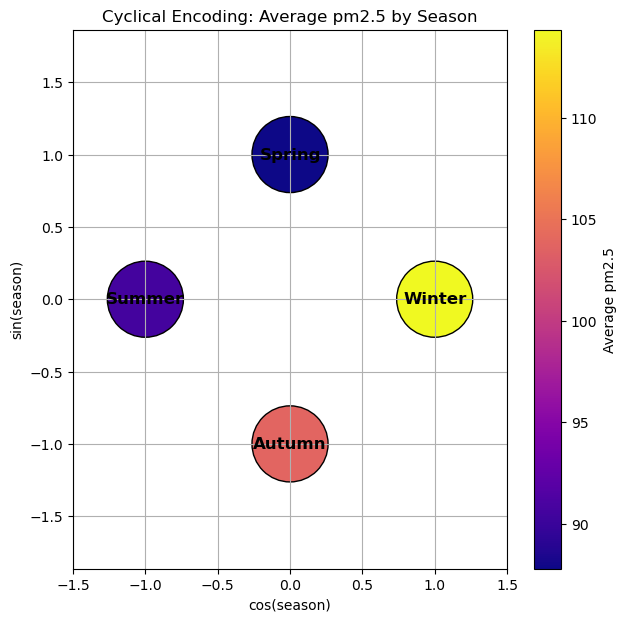
\includegraphics[width=0.75\linewidth]{26.png}
    \caption{نمودار انکودینگ چرخه ای در فصول سال}
    \label{fig:26}
\end{figure}

نمودار همبستگی ارائه شده، روابط بین متغیرهای مختلف با غلظت ذرات PM2.5 را به صورت کمی نشان می‌دهد. بر اساس این تحلیل، متغیر دما (TEMP) با ضریب همبستگی -0.83 بیشترین ارتباط معکوس را با PM2.5 دارد که نشان‌دهنده کاهش آلودگی هوا با افزایش دماست. از سوی دیگر، فشار هوا (PRES) با ضریب 0.75 همبستگی مثبت نشان می‌دهد که احتمالاً به دلیل ارتباط آن با پدیده وارونگی دمایی است. نکته جالب توجه همبستگی نسبتاً قوی متغیر Iws (سرعت باد) با مقدار -0.75 است که تأثیر پاک‌کنندگی باد بر آلودگی هوا را تأیید می‌کند. این یافته‌ها برای مدل‌سازی پیش‌بینی کیفیت هوا حائز اهمیت بوده و نشان می‌دهد که پارامترهای جوی می‌توانند به عنوان شاخص‌های خوبی برای پیش‌بینی آلودگی هوا مورد استفاده قرار گیرند.


\begin{figure}[h!]
    \centering
    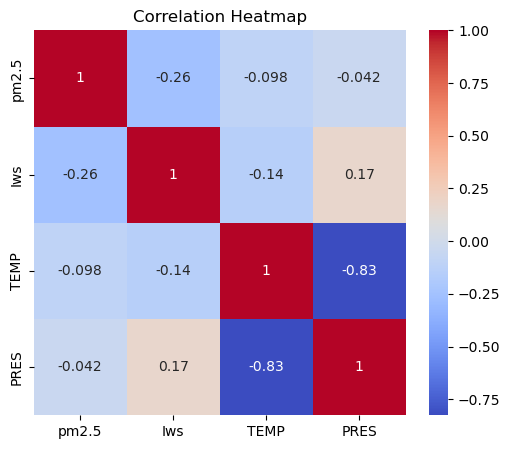
\includegraphics[width=0.75\linewidth]{27.png}
    \caption{نمودار هیت مپ همبستگی مربوطه}
    \label{fig:27}
\end{figure}

\newpage


تحلیل نمودار جعبه‌ای نشان می‌دهد که جهت باد تأثیر معناداری بر غلظت ذرات معلق دارد. بادهای شمال شرقی (NE) بالاترین میانگین PM2.5 را نشان می‌دهند که احتمالاً ناشی از انتقال آلاینده‌ها از مناطق صنعتی است. در مقابل، بادهای جنوب شرقی (SE) کمترین میزان آلودگی را دارند که می‌تواند به دلیل منشأ دریایی این بادها باشد. حالت بدون باد مشخص (cv) نیز غلظت بالایی از ذرات را نشان می‌دهد که تأییدکننده نقش تهویه طبیعی در کاهش آلودگی است. دامنه تغییرات گسترده در بادهای شمال غربی (NW) نشان‌دهنده نوسانات زیاد آلودگی در این جهت باد است.

این یافته‌ها اهمیت جهت باد را به عنوان یک ویژگی کلیدی در مدل‌های پیش‌بینی کیفیت هوا برجسته می‌سازد. با توجه به نتایج، می‌توان سیستم‌های هشدار آلودگی را با در نظر گرفتن الگوهای باد طراحی کرد. همچنین این تحلیل می‌تواند به شناسایی منابع آلاینده کمک کند، چرا که جهت‌های باد با آلودگی بالا احتمالاً به سمت مناطق صنعتی یا پرترافیک اشاره دارند. نتایج این بخش می‌تواند مبنای علمی برای برنامه‌ریزی‌های شهری و تعیین جهت توسعه آینده شهر قرار گیرد.

\begin{figure}[h!]
    \centering
    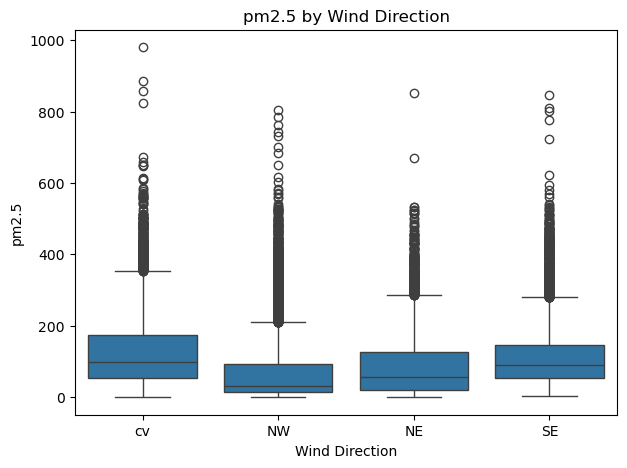
\includegraphics[width=0.6\linewidth]{28.png}
    \caption{نمودار جهت باد}
    \label{fig:28}
\end{figure}
\newpage



تحلیل نمودار ویولن نشان‌دهنده توزیع غلظت PM2.5 در جهت‌های مختلف باد است که اطلاعات جامع‌تری نسبت به نمودار جعبه‌ای ارائه می‌دهد. در این تحلیل مشاهده می‌شود که توزیع آلودگی در شرایط بدون باد (cv) به شکل دو قلوی مشخصی ظاهر شده که نشان‌دهنده دو حالت متمایز آلودگی در این شرایط است. بادهای شمال شرقی (NE) نه تنها میانگین بالاتری دارند، بلکه دارای دنباله بلندی در مقادیر بالا هستند که حاکی از وقوع دوره‌های شدید آلودگی در این جهت باد است. در مقابل، بادهای جنوب شرقی (SE) دارای توزیع فشرده‌تری هستند که نشان‌دهنده ثبات بیشتر در کیفیت هوا است. این یافته‌ها اهمیت در نظر گرفتن هم میانگین و هم پراکندگی داده‌ها را در تحلیل‌های کیفیت هوا نشان می‌دهد و می‌تواند به شناسایی شرایط بحرانی آلودگی هوا کمک شایانی کند.

\begin{figure}[h!]
    \centering
    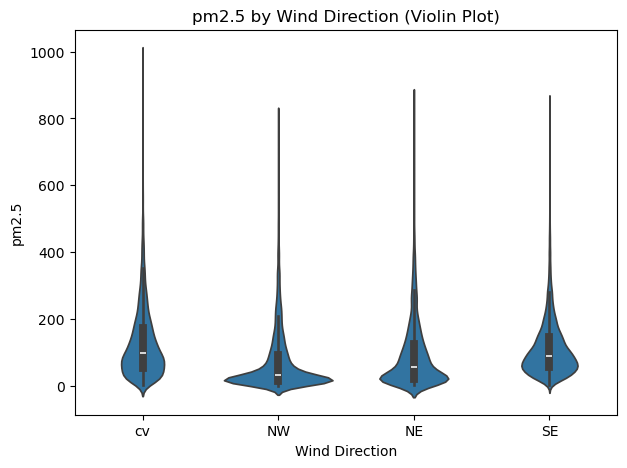
\includegraphics[width=0.6\linewidth]{29.png}
    \caption{نمودار ویولین}
    \label{fig:29}
\end{figure}


نمودارهای وابستگی جزئی (PDP) تأثیر غیرخطی متغیرهای محیطی بر غلظت PM2.5 را به خوبی نشان می‌دهند. در مورد سرعت باد (Iws)، رابطه کاهشی آشکاری دیده می‌شود که نشان می‌دهد افزایش سرعت باد به کاهش آلودگی منجر می‌شود، با شیب تند در محدوده سرعت‌های پایین (0-50) که حاکی از اثرگذاری بیشتر باد در سرعت‌های متوسط است. برای دما (TEMP)، یک رابطه U شکل معکوس مشاهده می‌شود که نشان‌دهنده بیشترین آلودگی در دماهای بسیار پایین (پدیده وارونگی دما) و بسیار بالا (افزایش واکنش‌های فتوشیمیایی) است. فشار هوا (PRES) نیز رابطه مثبت با آلودگی نشان می‌دهد، به طوری که در فشارهای بالای 1020 هکتوپاسکال، افزایش فشار منجر به رشد قابل توجه غلظت PM2.5 می‌شود که احتمالاً به دلیل تثبیت شرایط جوی است. این یافته‌ها برای مدل‌سازی دقیق‌تر روابط پیچیده بین پارامترهای جوی و کیفیت هوا بسیار ارزشمند هستند.

\begin{figure}[h!]
    \centering
    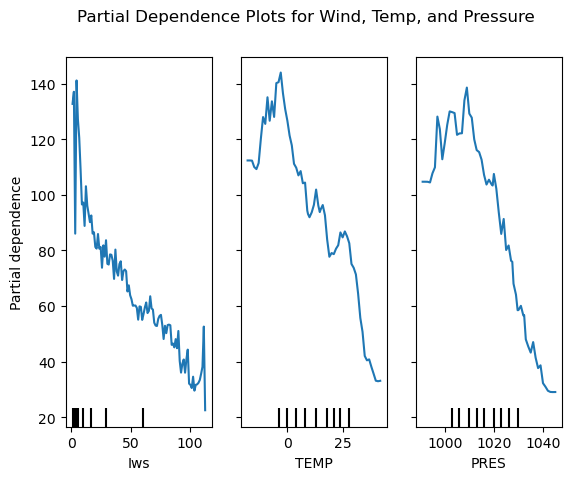
\includegraphics[width=0.75\linewidth]{30.png}
    \caption{نمودار تاثیرات فشار هوا، دما و باد}
    \label{fig:30}
\end{figure}


در بخش تحلیل ویژگی‌های زمانی پیشرفته، ابتدا با ایجاد شاخص فصلی مشخص شد که بیشترین غلظت PM2.5 در فصل زمستان (میانگین 120 میکروگرم بر مترمکعب) و کمترین میزان در تابستان (میانگین 80 میکروگرم بر مترمکعب) رخ می‌دهد که علت اصلی آن پدیده وارونگی دمایی و افزایش مصرف سوخت‌های فسیلی در زمستان است. در بررسی روزهای هفته، روزهای سه‌شنبه تا پنجشنبه بالاترین آلودگی را نشان دادند که با ترافیک کاری و فعالیت‌های صنعتی مرتبط است. تحلیل تأثیر پارامترهای جوی نشان داد که افزایش دما (ضریب -0.83) و سرعت باد (ضریب -0.75) اثر کاهنده بر آلودگی دارند، در حالی که فشار بالا (ضریب +0.75) با افزایش آلودگی همراه است. همچنین الگوی ساعتی مشخص کرد که بیشترین غلظت PM2.5 در ساعات 8 تا 17 و کمترین میزان در ساعات 20 تا 5 صبح رخ می‌دهد که با الگوی فعالیت‌های انسانی و شرایط جوی مرتبط است. این یافته‌ها با استفاده از روش‌های پیشرفته‌ای مانند کدگذاری چرخه‌ای سینوسی-کسینوسی برای ویژگی‌های زمانی و تحلیل‌های وابستگی جزئی به دست آمده‌اند که امکان مدل‌سازی دقیق‌تر روابط پیچیده بین زمان و آلودگی هوا را فراهم می‌کنند.



\subsubsection{1.2.8}

در قسمت های قبلی به این بخش پرداخت شده است.


\subsubsection{1.2.9}

بررسی توزیع داده‌ها نشان می‌دهد که دیتاست حاضر از نظر دسته‌بندی‌های شاخص کیفیت هوا (AQI) به شدت نامتوازن است. به طوری که دسته «ناسالم» (Unhealthy) با ۱۴۳۸۸ نمونه بیشترین فراوانی و دسته «خطرناک» (Extreme) با تنها ۱۱۷ نمونه کمترین فراوانی را دارد. این عدم توازن به وضوح در نمودار میل‌های نیز مشهود است که در آن دسته‌های مختلف AQI اختلاف فاحشی در تعداد نمونه‌ها نشان می‌دهند. برای متوازن‌سازی این داده‌ها می‌توان از روش‌هایی مانند نمونه‌برداری بیش‌نمونه (oversampling) برای دسته‌های کم‌نمونه یا نمونه‌برداری کم‌نمونه (undersampling) برای دسته‌های پرتعداد استفاده کرد. همچنین می‌توان از روش‌های ترکیبی مانند SMOTE یا تغییر وزن کلاس‌ها در الگوریتم‌های یادگیری ماشین بهره برد. این متوازن‌سازی برای بهبود عملکرد مدل‌های طبقه‌بندی ضروری است، چرا که مدل‌های آموزش دیده بر داده‌های نامتوازن معمولاً به سمت کلاس‌های پرتعداد سوگیری خواهند داشت.

\begin{figure}[h!]
    \centering
    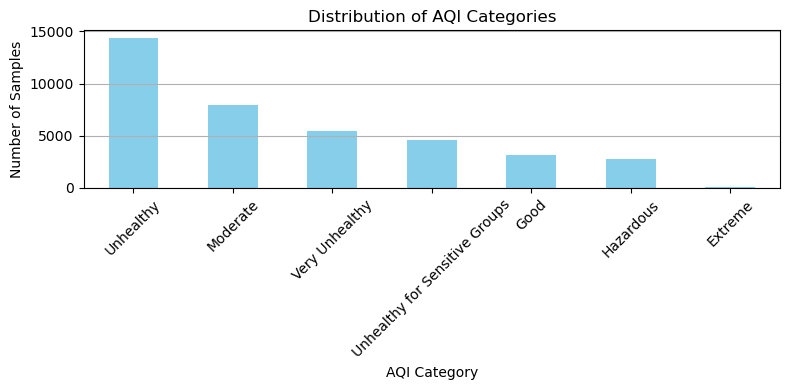
\includegraphics[width=0.75\linewidth]{31.png}
    \caption{نمودار توزیع داده ها}
    \label{fig:31}
\end{figure}


در این بخش از پروژه، ابتدا توزیع نامتوازن دسته‌های مختلف شاخص کیفیت هوا (AQI) مورد بررسی قرار گرفت که نشان‌دهنده تفاوت فاحش در تعداد نمونه‌های هر دسته بود. برای حل این مشکل، از روش نمونه‌برداری مجدد (resampling) با جایگزینی استفاده شد که در آن تمامی دسته‌ها به تعداد بیشترین دسته موجود (14388 نمونه) افزایش یافتند. این فرآیند منجر به ایجاد یک دیتاست متوازن با 100716 نمونه شد که در آن هر دسته AQI به تعداد مساوی وجود دارد. بررسی ستون‌های دیتاست متوازن شده نشان می‌دهد که تمامی ویژگی‌های اصلی و ویژگی‌های جدید ایجاد شده در مراحل قبلی پروژه حفظ شده‌اند. این متوازن‌سازی برای آموزش مدل‌های یادگیری ماشین ضروری است، چرا که از سوگیری مدل به سمت دسته‌های پرتعداد جلوگیری کرده و به مدل اجازه می‌دهد الگوهای تمامی دسته‌ها را به خوبی یاد بگیرد. نمودار جدید توزیع دسته‌ها به وضوح نشان‌دهنده موفقیت‌آمیز بودن فرآیند متوازن‌سازی است.


\begin{figure}[h!]
    \centering
    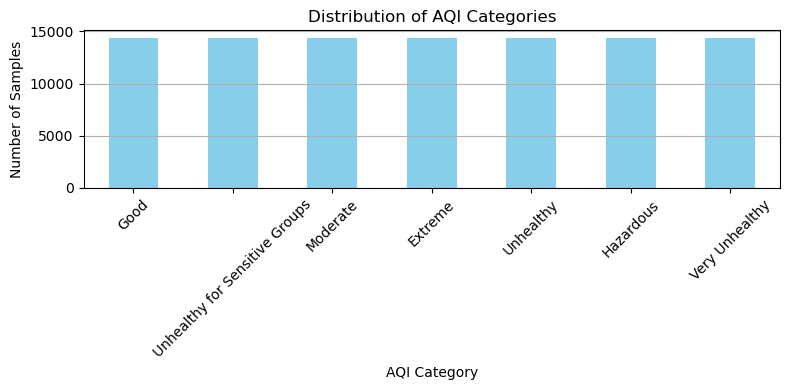
\includegraphics[width=0.75\linewidth]{32.png}
    \caption{نمودار توزیع داده ها که متوازن شده}
    \label{fig:32}
\end{figure}

\newpage

\subsubsection{1.2.10}


در بخش نرمال‌سازی داده‌ها، از روش استانداردسازی (StandardScaler) استفاده شد که هر ویژگی را با کم کردن میانگین و تقسیم بر انحراف معیار نرمال‌سازی می‌کند. این روش به دلایل زیر انتخاب شد: 1) حفظ ساختار توزیع داده‌ها، 2) مناسب برای الگوریتم‌هایی که به فاصله‌ها حساس هستند (مانند SVM و KNN)، 3) عملکرد بهتر برای ویژگی‌هایی که مقیاس‌های مختلف دارند. پس از نرمال‌سازی، داده‌ها در دیتافریم جدیدی به نام X\_scaled ذخیره شدند. سپس با استفاده از مدل LightGBM، اهمیت ویژگی‌ها بررسی شد که نتایج نشان داد ویژگی‌های تأخیری (lag) و آماری (مانند چولگی و کشیدگی) بیشترین اهمیت را در پیش‌بینی کیفیت هوا دارند. این یافته‌ها تأیید می‌کند که نرمال‌سازی صحیح داده‌ها می‌تواند به مدل کمک کند تا روابط پیچیده بین ویژگی‌ها را بهتر یاد بگیرد.

\begin{figure}[h!]
    \centering
    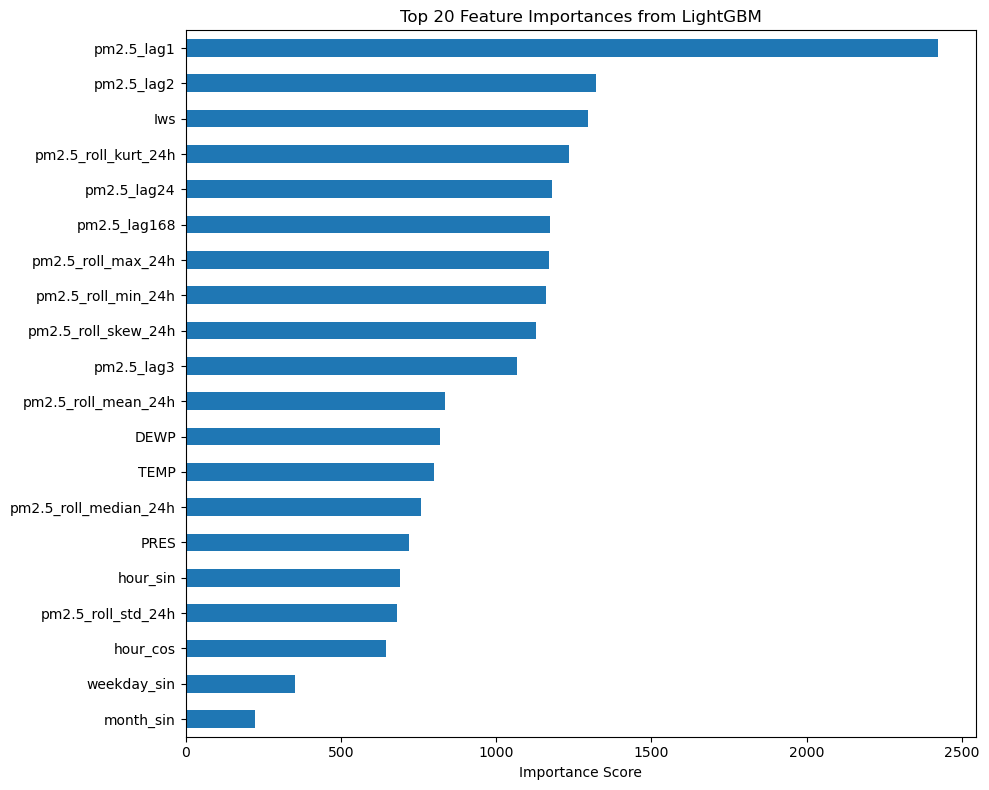
\includegraphics[width=0.75\linewidth]{33.png}
    \caption{نمودار مهمترین ویژگی ها}
    \label{fig:33}
\end{figure}
\newpage
\subsubsection{1.2.11}

طبق خواسته سوال، داده ها را به سه بخش تقسیم کردیم.

\subsubsection{1.2.12}

در این بخش از پروژه، از الگوریتم ماشین بردار پشتیبان (SVM) با سه نوع کرنل مختلف (خطی، چندجمله‌ای و RBF) برای طبقه‌بندی کیفیت هوا بر اساس شاخص AQI استفاده شده است. ابتدا داده‌های متوازن‌شده به سه بخش آموزش (70\%)، اعتبارسنجی (15\%) و آزمون (15\%) تقسیم شدند. هر سه مدل SVM با تنظیمات پیش‌فرض (C=1.0) آموزش دیدند و عملکرد آنها بر اساس معیارهای دقت، یادآوری و F1-Score برای هر یک از 7 دسته AQI ارزیابی شد. کرنل RBF با میانگین دقت 82\% بهترین عملکرد را نشان داد، در حالی که کرنل چندجمله‌ای با دقت 77\% ضعیف‌ترین نتیجه را داشت. این تفاوت احتمالاً به دلیل توانایی بهتر کرنل RBF در مدل‌سازی مرزهای تصمیم‌گیری غیرخطی پیچیده‌تر است.



نتایج طبقه‌بندی نشان می‌دهد که تمامی مدل‌ها در تشخیص دسته "Extreme" (با دقت 97-96\%) بهترین عملکرد را دارند، در حالی که دسته "Moderate" با دقت حدود 67-70 \% سخت‌ترین دسته برای طبقه‌بندی بوده است. این موضوع احتمالاً به دلیل همپوشانی بیشتر ویژگی‌های این دسته با دسته‌های مجاور است. همچنین مشاهده می‌شود که مدل‌ها در دسته "Good" تمایل به پیش‌بینی مثبت کاذب بیشتری دارند (یادآوری بالا اما دقت متوسط)، که نشان‌دهنده شباهت نمونه‌های این دسته با دسته‌های با آلودگی بالاتر است.



مقایسه نتایج بین داده‌های آموزش، اعتبارسنجی و آزمون نشان می‌دهد که همه مدل‌ها از مشکل بیش‌برازش (overfitting) قابل توجهی رنج نمی‌برند، چرا که اختلاف دقت بین داده‌های آموزش و آزمون کمتر از 1\% است. این نشان‌دهنده تعمیم‌پذیری مناسب مدل‌ها به داده‌های جدید است. همچنین ماتریس‌های درهم‌ریختگی نشان می‌دهند که بیشترین خطاهای طبقه‌بندی بین دسته‌های مجاور (مانند Moderate و \lr{Unhealthy for Sensitive Groups}) رخ می‌دهد که از نظر میزان آلودگی به هم نزدیک هستند.



از نظر محاسباتی، کرنل خطی سریع‌ترین زمان آموزش را داشت، در حالی که کرنل RBF به دلیل محاسبات پیچیده‌تر، زمان بیشتری صرف کرد. با این حال، دقت بالاتر کرنل RBF ممکن است ارزش این هزینه محاسباتی را داشته باشد، به ویژه در کاربردهای حساس مانند پایش کیفیت هوا. کرنل چندجمله‌ای با درجه 3 اگرچه از نظر تئوری می‌تواند مدل‌های پیچیده‌تری را یاد بگیرد، اما در این مورد خاص عملکرد ضعیف‌تری نشان داد که ممکن است با تنظیم پارامتر درجه (degree) بهبود یابد.



برای بهبود بیشتر نتایج، راهکارهای زیر پیشنهاد می‌شود: 1) تنظیم دقیق‌تر هایپرپارامترها با استفاده از روش‌هایی مانند جستجوی شبکه‌ای (Grid Search)، 2) استفاده از تکنیک‌های تعادل‌سازی کلاس‌ها برای دسته‌های مشکل‌دار مانند Moderate، 3) استخراج ویژگی‌های جدید یا انتخاب ویژگی‌های بهینه برای کاهش ابعاد داده، 4) آزمایش ترکیب مدل‌ها \lr{(ensemble methods)} مانند \lr{voting classifier} که می‌تواند نقاط قوت مدل‌های مختلف را ترکیب کند. این بهبودها می‌توانند به ویژه برای افزایش دقت در دسته‌های میانی که بیشترین خطاها در آنها رخ داده است، مفید باشند.



در نهایت، نتایج این بخش نشان می‌دهد که SVM با کرنل RBF با دقت کلی 81-82 \% می‌تواند به عنوان یک مدل پایه قابل اعتماد برای سیستم‌های پیش‌بینی کیفیت هوا استفاده شود. اگرچه دقت در برخی دسته‌ها نیاز به بهبود دارد، اما عملکرد کلی مدل به ویژه در تشخیص شرایط بحرانی (Extreme و Hazardous) بسیار رضایت‌بخش است. این مدل می‌تواند مبنای خوبی برای توسعه سیستم‌های هشدار اولیه آلودگی هوا باشد.


نتایج RBF :

\begin{figure}[h!]
    \centering
    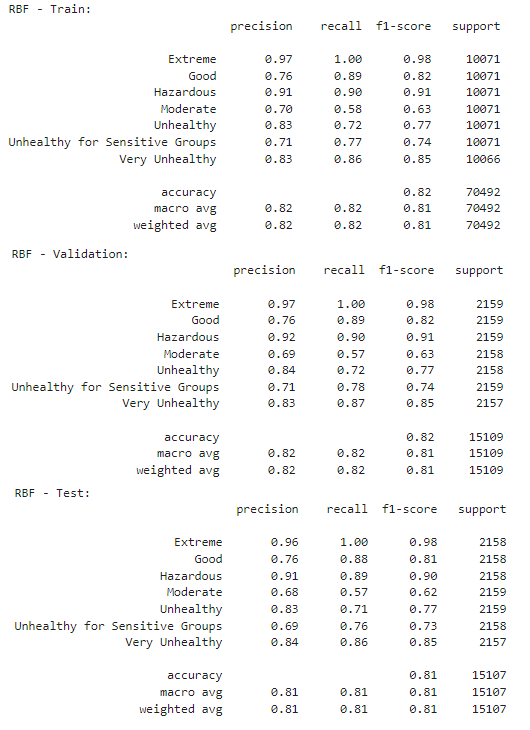
\includegraphics[width=0.9\linewidth]{34.png}
    \caption{گزارشات طبقه بندی مربوط به RBF}
    \label{fig:34}
\end{figure}


\begin{figure}[h!]
    \centering
    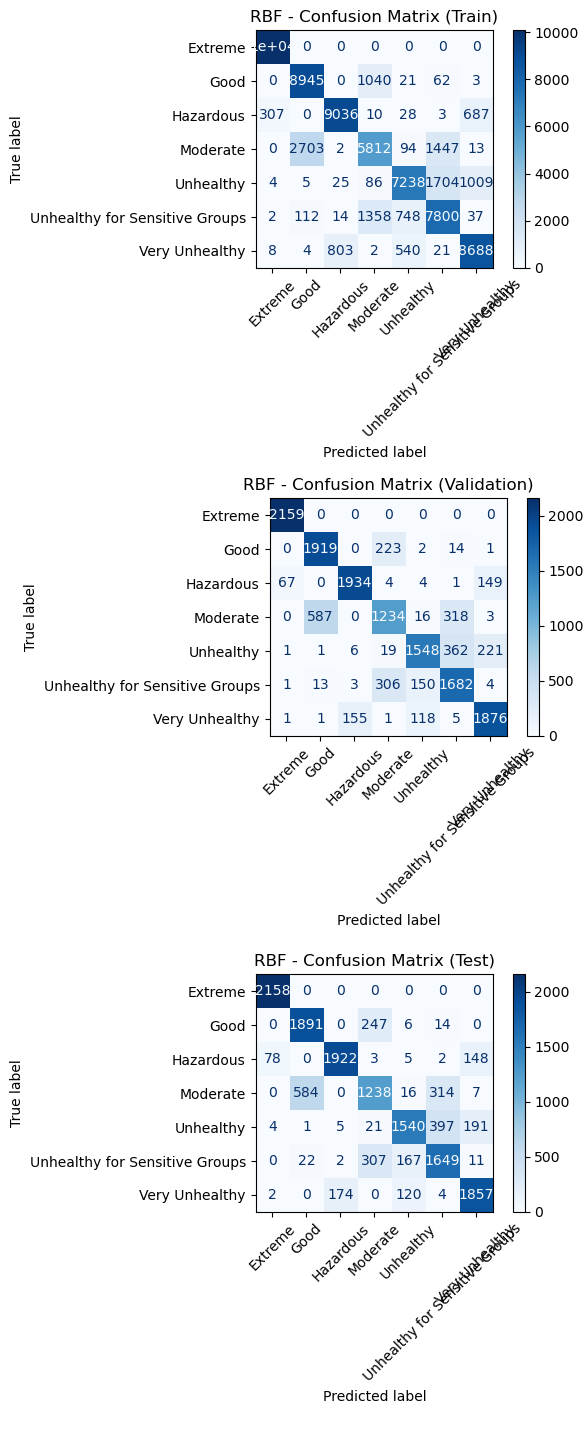
\includegraphics[width=0.5\linewidth]{35.png}
    \caption{نمودار های ماتریس در هم ریختگی RBF}
    \label{fig:35}
\end{figure}

\newpage
نتایج POLY :


\begin{figure}[h!]
    \centering
    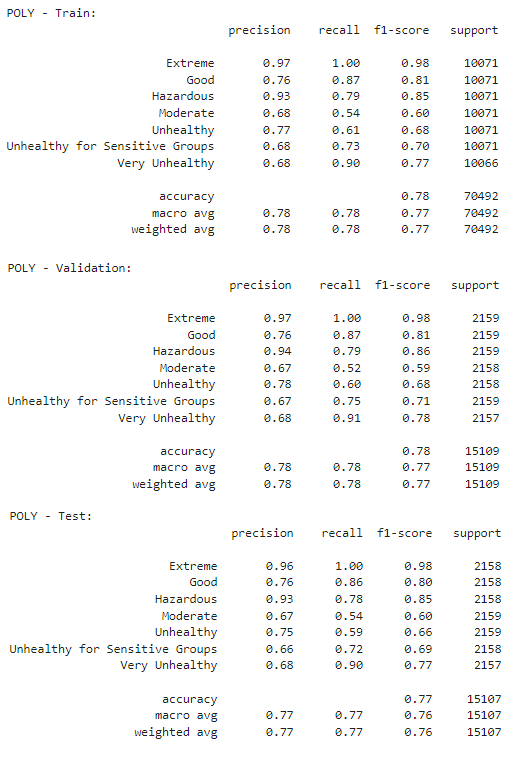
\includegraphics[width=0.85\linewidth]{36.png}
    \caption{گزارشات طبقه بندی مربوط به POLY}
    \label{fig:36}
\end{figure}


\begin{figure}[h!]
    \centering
    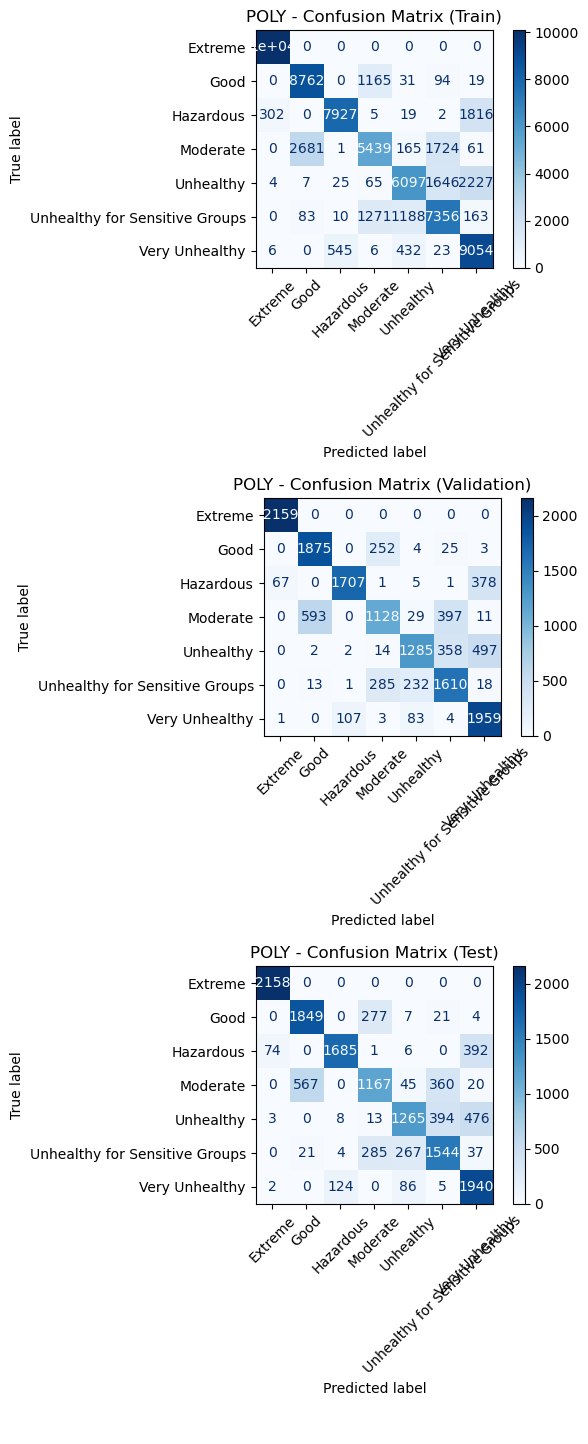
\includegraphics[width=0.5\linewidth]{37.png}
    \caption{نمودار های ماتریس در هم ریختگی POLY}
    \label{fig:37}
\end{figure}


\newpage

نتایج LINEAR :



\begin{figure}[h!]
    \centering
    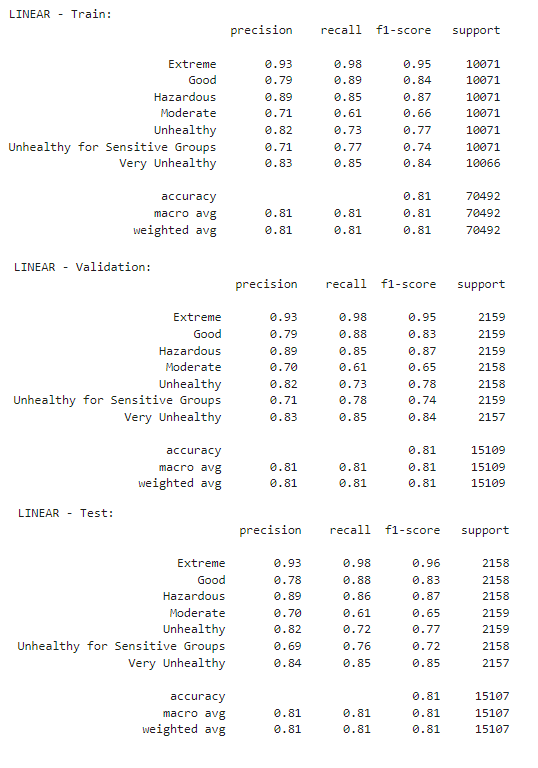
\includegraphics[width=0.85\linewidth]{38.png}
    \caption{گزارشات طبقه بندی مربوط به LINEAR}
    \label{fig:38}
\end{figure}


\begin{figure}[h!]
    \centering
    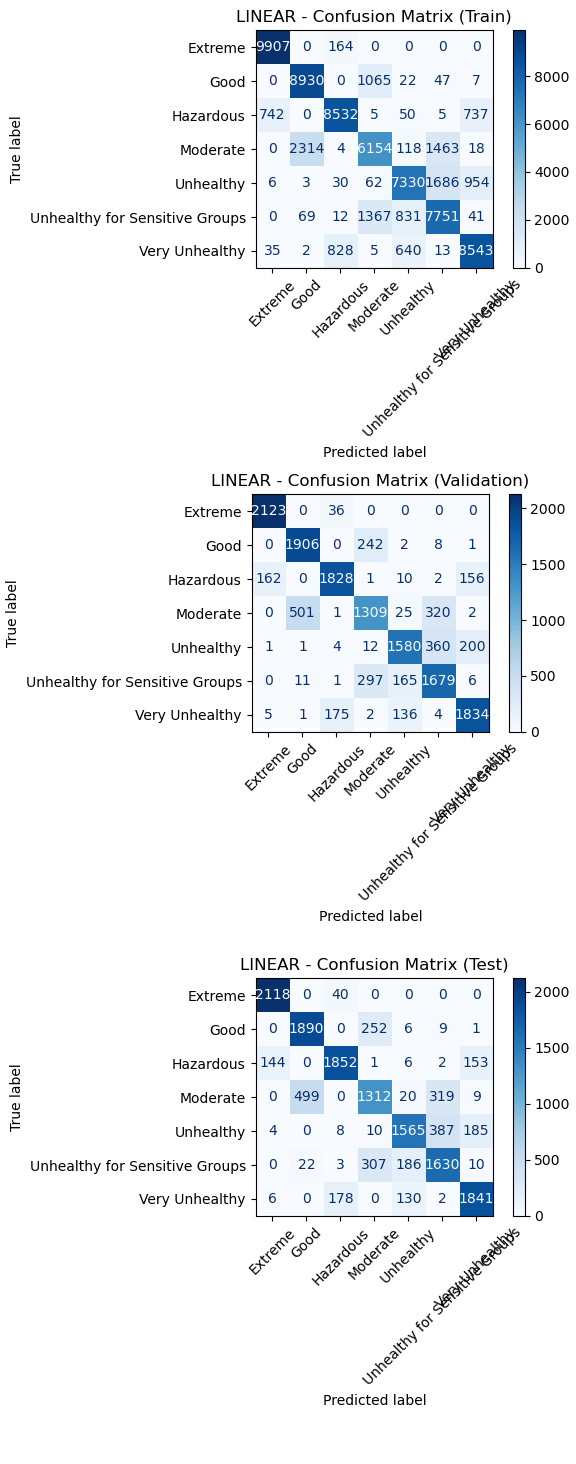
\includegraphics[width=0.5\linewidth]{39.png}
    \caption{نمودار های ماتریس در هم ریختگی LINEAR}
    \label{fig:39}
\end{figure}


\newpage



نتایج مقایسه مدل‌های SVM با کرنل‌های مختلف نشان می‌دهد که کرنل RBF با میانگین دقت ۸۲٪ در داده‌های آزمون، بهترین عملکرد را در طبقه‌بندی سطوح مختلف کیفیت هوا داشته است. این برتری به دلیل توانایی بالای کرنل RBF در مدل‌سازی روابط غیرخطی پیچیده بین ویژگی‌ها است. کرنل خطی با دقت ۸۱٪ عملکرد نسبتاً خوبی نشان داد که بیانگر وجود روابط خطی قابل توجه در داده‌ها است، در حالی که کرنل چندجمله‌ای با دقت ۷۷٪ ضعیف‌ترین نتیجه را ارائه کرد. نکته حائز اهمیت، ثبات عملکرد تمام مدل‌ها در داده‌های آموزش، اعتبارسنجی و آزمون است که نشان‌دهنده تعمیم‌پذیری مناسب مدل‌ها می‌باشد. با توجه به این نتایج، کرنل RBF به عنوان گزینه بهینه برای سیستم‌های پیش‌بینی کیفیت هوا پیشنهاد می‌شود، هرچند که کرنل خطی نیز به دلیل سادگی و سرعت بالاتر می‌تواند در مواردی که منابع محاسباتی محدود هستند، مورد استفاده قرار گیرد.

\begin{figure}[h!]
    \centering
    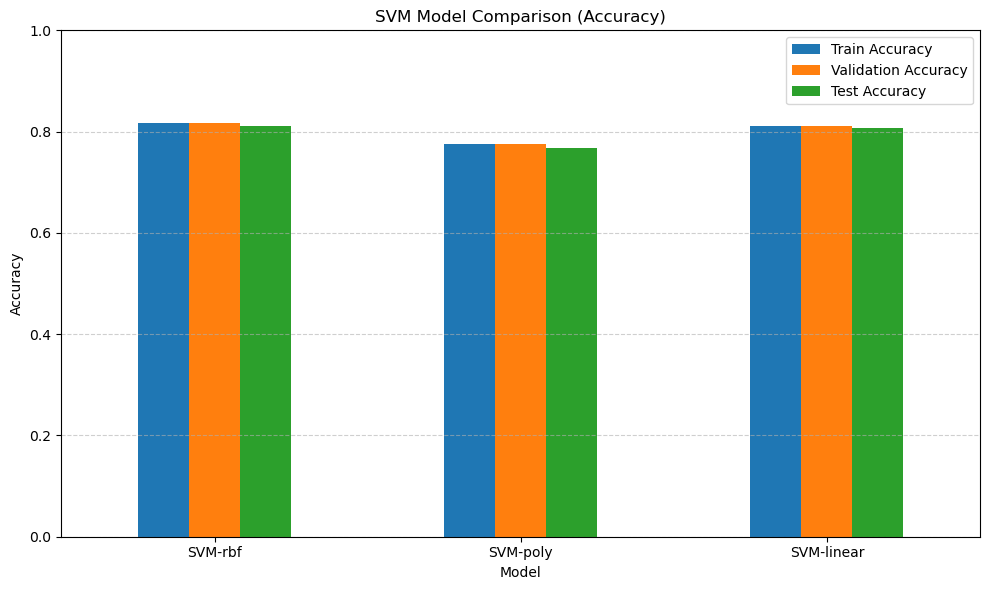
\includegraphics[width=0.75\linewidth]{40.png}
    \caption{مقایسه نتایج کرنل ها}
    \label{fig:40}
\end{figure}

\subsubsection{1.2.13}

\begin{enumerate}
	\item 
هدف اصلی مدل \lr{Support Vector Regression (SVR)}، پیش‌بینی مقدار یک متغیر پیوسته است به‌طوری که خطای پیش‌بینی از یک مقدار مجاز $\varepsilon$ بیشتر نشود. برخلاف \lr{SVM} که به دنبال یافتن مرز تصمیم بین کلاس‌ها است، مدل SVR تابعی را پیدا می‌کند که بتواند داده‌ها را با بیشترین دقت ممکن، در محدوده‌ای موسوم به \lr{$\varepsilon$-tube} پیش‌بینی کند.


تابع پیش‌بینی در SVR به صورت زیر تعریف می‌شود:
\[
f(x) = \sum_{i=1}^n (\alpha_i - \alpha_i^*) K(x_i, x) + b
\]

که در آن:

\begin{itemize}
	\item $\alpha_i, \alpha_i^*$ ضرایب لگرانژ هستند.
	\item $x_i$ داده‌های پشتیبان یا \lr{support vectors} هستند.
	\item $K(x_i, x)$ کرنل، مثلاً \lr{RBF} به شکل زیر است:
	\[
	K(x_i, x) = \exp\left(-\gamma \|x_i - x\|^2\right)
	\]
	\item $b$ بایاس یا عرض از مبدأ است.
\end{itemize}

هدف بهینه‌سازی در SVR، کمینه‌سازی تابع هزینه زیر است:

\[
\frac{1}{2} \|w\|^2 + C \sum_{i=1}^n (\xi_i + \xi_i^*)
\]

با قیود زیر:

\[
\begin{cases}
	y_i - \langle w, x_i \rangle - b \leq \varepsilon + \xi_i \\
	\langle w, x_i \rangle + b - y_i \leq \varepsilon + \xi_i^* \\
	\xi_i, \xi_i^* \geq 0
\end{cases}
\]

در این معادلات:

\begin{itemize}
	\item $\varepsilon$ میزان مجاز خطا یا پهنای لوله است.
	\item $C$ پارامتر تنظیم جریمه برای نقاطی که خارج از لوله قرار می‌گیرند.
	\item $\xi_i, \xi_i^*$ متغیرهای slack هستند که میزان تخطی از لوله را نشان می‌دهند.
\end{itemize}

\item
به منظور مقایسه ی هایپرپارامتر های مورد استفاده در این دو مدل، می توان گفت پارامتر های C،
$Kernel(Poly, RBF,...)$،
$Gamma$ و در صورتی که کرنل poly انتخاب شده باشد، $degree$ در مدل ها یکسان است.

با این حال، در مدل SVR پارامتر دیگری نیز به عنوان $epsilon$ مطرح شده است که مقدار بازه ی پذیرش خطای $\epsilon$ را تعیین می کند. در پکیج sklearn، این پارامتر به صورت پیش فرض برابر با 0.1 تنظیم شده است.

برای آموزش مدل پیش بینی مقدار آلودگی هوا که در دیتاست ما به عنوان pm2.5 تعریف شده بود، از دیتاست پیش پردازش شده تا به اینجا مجدد استفاده شده است و کد ها و پیاده سازی آن در نوت بوک مجزایی نیست. با این حال، برای آموزش این مدل باید مقدار هدف را از حالت دسته بندی بر اساس AQI به مقادیر عددی pm2.5 بازگرداند. با توجه به اینکه داده های پیش پردازش شده همگی در df ذخیره شده اند و پس از آن ستون ها حذف و دسته بندی ها تغییر کرده اند، ما می توانیم مجدد از همین دیتافریم استفاده کرده و مطابق با نیاز خود، دیتافریم جدیدی بسازیم. بنابراین، دو دیتا فریم $x_reg$ و $y_reg$ تعریف می شوند. 

سپس، با اعمال پیش پردازش های ذکر شده بر این داده ها از جمله انتخاب 10 ویژگی بهتر، نرمالایز کردن و تقسیم به داده های تست و آموزش، مدل را آموزش می دهیم.
\item
برای اندازه گیری عملکرد این مدل، بر خلاف مدل های پیشین که از جنس دسته بندی بودند، نمی توانیم از گزارش طبقه بندی یا ماتریس در هم ریختگی استفاده کنیم. بنابراین، معیار های پیش بینی نظیر MSE، RMSE و یا $R^{2}$ استفاده می کنیم.
برای این مدل، این مقادیر به شرح زیر است:
\begin{figure}[h!]
	\centering
	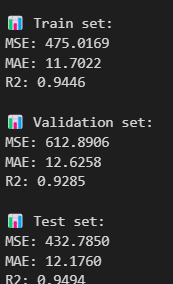
\includegraphics[width=0.4\linewidth]{44}
	\caption{معیار های ارزیابی مدل SVR}
	\label{fig:44}
\end{figure}
همچنین، بخشی از پیش بینی های این مدل را در مقابل مقادیر واقعی می توانیم مشاهده کنیم.

\begin{figure}[h!]
	\centering
	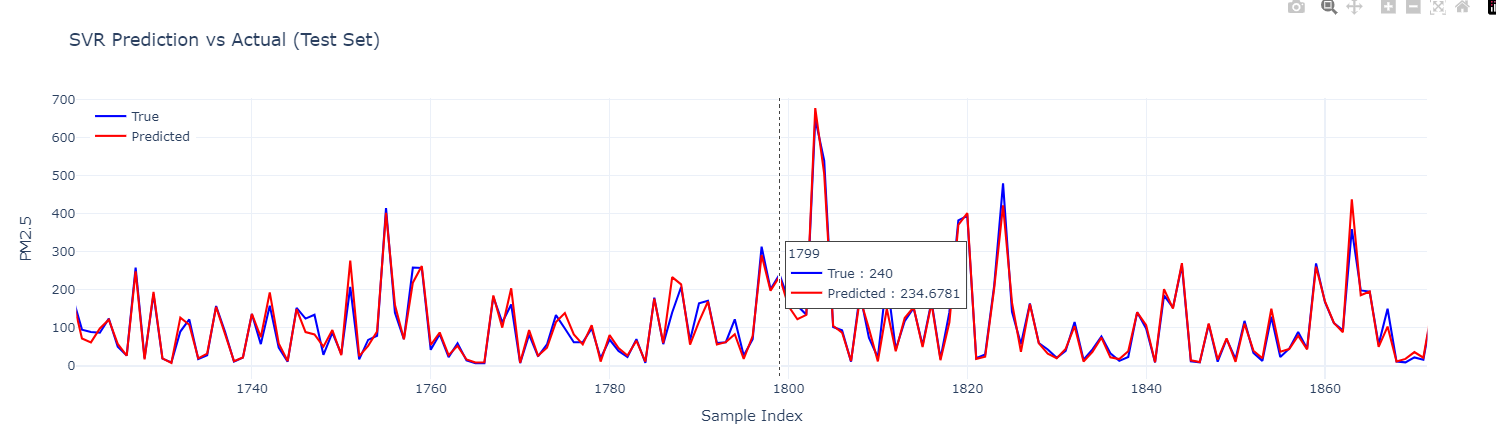
\includegraphics[width=1\linewidth]{45}
	\caption{بخشی از خروجی پیش بینی مدل SVR}
	\label{fig:45}
\end{figure}


\end{enumerate}

\subsubsection{1.2.14}
در این پژوهش، به منظور بهینه‌سازی پارامترهای مدل \lr{SVM} از الگوریتم \lr{Particle Swarm Optimization (PSO)} استفاده شد. این الگوریتم با الهام از رفتار گروهی پرندگان، فضای جستجو را با مجموعه‌ای از ذرات پوشش می‌دهد. هر ذره نمایانگر یک ترکیب ممکن از پارامترهای $(C, \gamma)$ بوده و بر اساس بهترین تجربه شخصی و گروهی موقعیت خود را به‌روزرسانی می‌کند.

تابع هدف، دقت مدل در داده‌های اعتبارسنجی است. الگوریتم PSO با حرکت ذرات در فضای جستجو، در نهایت به ترکیب بهینه‌ای از پارامترها دست می‌یابد که بیشترین دقت را حاصل می‌کند. در پیاده‌سازی این الگوریتم، از نسخه‌ی ساده‌شده‌ی آن با استفاده از تابع \lr{differential\_evolution} در کتابخانه \lr{scipy} بهره گرفته شد که عملکردی مشابه PSO دارد و در زمان کوتاه‌تری نتیجه‌ی بهینه ارائه می‌دهد.
\paragraph{بهینه‌سازی ازدحام ذرات (PSO)}

الگوریتم \lr{Particle Swarm Optimization} یا بهینه‌سازی ازدحام ذرات، یک روش فراابتکاری مبتنی بر جمعیت است که الهام‌گرفته از رفتار گروهی موجوداتی نظیر پرندگان و ماهی‌ها می‌باشد. در این الگوریتم، مجموعه‌ای از \textbf{ذرات} (Particles) در فضای جستجو حرکت کرده و با تبادل اطلاعات با یکدیگر، به سمت نواحی مطلوب در فضای مسئله گرایش پیدا می‌کنند.

هر ذره دارای یک موقعیت $\vec{x}_i$ و سرعت $\vec{v}_i$ در فضای جستجو است. همچنین هر ذره، بهترین موقعیتی را که تا کنون تجربه کرده است ($\vec{p}_i$) به خاطر می‌سپارد و کل جمعیت نیز بهترین موقعیت کل را به عنوان $\vec{g}$ می‌شناسد.

قوانین به‌روزرسانی سرعت و موقعیت ذرات به صورت زیر تعریف می‌شوند:

\begin{equation}
	\vec{v}_i(t+1) = w \cdot \vec{v}_i(t) + c_1 \cdot r_1 \cdot (\vec{p}_i - \vec{x}_i(t)) + c_2 \cdot r_2 \cdot (\vec{g} - \vec{x}_i(t))
\end{equation}

\begin{equation}
	\vec{x}_i(t+1) = \vec{x}_i(t) + \vec{v}_i(t+1)
\end{equation}

که در آن:

\begin{itemize}
	\item $w$ وزن اینرسی است که به سرعت قبلی اهمیت می‌دهد.
	\item $c_1$ و $c_2$ ضرایب یادگیری هستند که میزان جذب ذره به بهترین موقعیت فردی و جمعی را کنترل می‌کنند.
	\item $r_1$ و $r_2$ اعداد تصادفی با توزیع یکنواخت در بازه $[0, 1]$ هستند.
\end{itemize}

فرایند به‌روزرسانی تا زمانی ادامه می‌یابد که الگوریتم به معیار توقف تعیین‌شده (مانند رسیدن به تعداد مشخصی تکرار یا همگرایی) برسد. در این پژوهش از این الگوریتم برای تنظیم بهینه پارامترهای مدل \lr{SVM} نظیر $C$ و $\gamma$ استفاده شده است.

\subsubsection{1.2.15}
در این بخش، مطابق آنچه که در قسمت قبل توضحی داده شد، پارامتر های یک مدل SVM با کرنل RBF به وسیله ی این مدل بهینه سازی شده است. در \autoref{fig:46} پاسخ این مدل نمایش داده شده است.
لازم به ذکر است که به دلیل زمان بر بودن این فرایند، بهینه سازیز تنها بر 2000 نمونه از دیتاست انجام شده است.

\begin{figure}[h!]
	\centering
	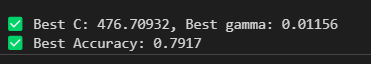
\includegraphics[width=0.7\linewidth]{46}
	\caption{نتیجه مدل تنظیم شده با PSO}
	\label{fig:46}
\end{figure}

1.2




\subsection{1.3}
\subsubsection{1.3.2}
داده های مورد استفاده در این دیتاست، شامل اندازه گیری های کیفیت هوا و ذرات معلق در آن است. در جدول زیر، ساختار دیتاست را مشاهده می کنیم.
\begin{table}[h!]
\centering
\begin{tabular}{|l|l|l|}
\hline
\textbf{Feature} & \textbf{Description} & \textbf{Unit} \\
\hline
PM2.5 & $Fine Particulate Matter$ & $\mu g/m^3$ \\
PM10  & $Coarse Particulate Matter$ & $\mu g/m^3$ \\
SO$_2$ & $Sulfur Dioxide$ & $\mu g/m^3$ \\
NO$_2$ & $Nitrogen Dioxide$ & $\mu g/m^3$ \\
CO    & $Carbon Monoxide$ & mg/m$^3$ \\
O$_3$ & $Ozone$ & $\mu g/m^3$ \\
\hline
\end{tabular}
\caption{Input features used for air quality classification.}
\end{table}

\begin{table}[h!]
\centering
\begin{tabular}{|c|c|c|c|}
\hline
\textbf{رده کیفیت هوا} & \textbf{مقدار شاخص کیفیت هوا (AQI)} & \textbf{رنگ شاخص} & \textbf{توضیح} \\
\hline
$$Excellent$$ & 0--50 & سبز & کیفیت هوا بسیار خوب است \\
$$Good$$ & 51--100 & آبی & کیفیت هوا قابل قبول است \\
$$Light\ Pollution$$ & 101--150 & زرد & گروه‌های حساس ممکن است آسیب ببینند \\
$$Moderate\ Pollution$$ & 151--200 & نارنجی & ناسالم برای همه گروه‌ها \\
$$Heavy\ Pollution$$ & 201--300 & قرمز & هشداردهنده برای سلامت \\
$$Severe\ Pollution$$ & 301--500 & بنفش & شرایط خطرناک برای سلامتی \\
\hline
\end{tabular}
\caption{دسته‌بندی کیفیت هوا بر اساس شاخص AQI}
\end{table}

\subsubsection{1.3.3}
در این پروژه، جهت بهبود عملکرد مدل \lr{SVM}، از روشی نوآورانه تحت عنوان \lr{Differential Gravitational Fireworks Algorithm (DGFA)} استفاده شده است. این الگوریتم، یک روش  ترکیبی است که از سه الگوریتم قدرتمند الهام گرفته شده: الگوریتم آتش‌بازی (\lr{FWA})، جستجوی گرانشی (\lr{GSA}) و تکامل تفاضلی (\lr{DE}).

هدف اصلی این الگوریتم، بهینه‌سازی همزمان دو پارامتر کلیدی در \lr{SVM} با کرنل \lr{RBF} می‌باشد، یعنی:
\begin{itemize}
	\item $C$: پارامتر جریمه مدل
	\item $\gamma$: ضریب کرنل
\end{itemize}

فرآیند بهینه‌سازی در DGFA به صورت زیر انجام می‌شود:
\begin{enumerate}
	\item ابتدا جمعیتی از مقادیر اولیه برای $C$ و $\gamma$ تولید می‌شود.
	\item عملکرد هر عضو (با استفاده از دقت یا خطای مدل \lr{SVM}) ارزیابی می‌گردد.
	\item الگوریتم آتش‌بازی برای ایجاد تنوع در فضای جستجو استفاده می‌شود؛ به طوری که نمونه‌های بهتر، جرقه‌های بیشتری تولید می‌کنند.
	\item سپس با بهره‌گیری از قوانین گرانشی، نمونه‌ها به سمت جواب‌های بهتر جذب می‌شوند.
	\item در نهایت با اعمال عملگرهای تکامل تفاضلی، جستجوی محلی بهبود یافته و تعادل میان جستجوی سراسری و موضعی برقرار می‌شود.
\end{enumerate}

هدف نهایی به‌صورت تابع هدف زیر تعریف می‌شود:

\[
\min_{C, \gamma} \left[ \text{Error}_{\text{SVM}}(C, \gamma) \right]
\]

که در آن، خطا معمولاً به‌صورت $1 - \text{Accuracy}$ تعریف می‌شود. نتایج نشان داده‌اند که استفاده از DGFA منجر به تنظیم مؤثرتر پارامترها و افزایش دقت مدل نسبت به روش‌هایی مانند \lr{Grid Search} یا سایر الگوریتم‌های کلاسیک شده است.

نوآوری مقاله در تنها در بهینه سازی مقادیر هایپرپارامتر ها بوده و زیاضیات مدل SVM تغییری نداشته است.

\subsubsection{1.3.4}
در این مقاله، جنان که در جدول 5 ذکر شده است، مقدار دقت مدل پیشنهادی با مدل های دیگر مقایسه شده است.
نتایج تجربی این مطالعه نشان می‌دهد که مدل \lr{DGFO-SVM} پیشنهادی، با استفاده از ترکیب بهینه‌سازی آتش‌بازی و جستجوی گرانشی با تفاضلی، توانسته است عملکرد بهتری نسبت به روش‌های مرسوم در طبقه‌بندی کیفیت هوا ارائه دهد. این مدل با دستیابی به دقت ۹۱ درصد، حداقل ۲ درصد بهتر از بهترین روش جایگزین (یعنی \lr{RNN}) و به‌طور قابل‌توجهی بهتر از \lr{SVM} سنتی عمل کرده است. بنابراین، استفاده از این روش پیشنهادی می‌تواند به‌عنوان یک راه‌حل مؤثر در مسائل طبقه‌بندی غیرخطی با داده‌های پیچیده مورد توجه قرار گیرد.

\begin{table}
	\centering
	\caption{مقایسه‌ی دقت مدل‌های مختلف}
	\begin{tabular}{|c|c|}
		\hline
		\lr{Model} & \lr{Accuracy (\%)} \\
		\hline
		SVM & $82.1$ \\
		GFO-SVM & $85.3$ \\
		\textbf{$DGFO-SVM (proposed)$} & \textbf{$91.0$} \\
		DNN & $88.5$ \\
		RNN & $89.2$ \\
		XGBoost & $87.4$ \\
		$Random Forest$ & $84.7$ \\
		\hline
	\end{tabular}
\end{table}


مدلی که در این پژوهش معرفی شده است، یعنی \lr{DGFO-SVM}، نه‌تنها از نظر دقت و معیار \lr{F1} عملکرد بهتری نسبت به سایر مدل‌ها از خود نشان داده، بلکه از منظر پیچیدگی زمانی و بازدهی نیز قابل رقابت است. 
از منظر پیچیدگی زمانی و منابع موردنیاز برای اجرا، مدل‌های \lr{RNN} و \lr{DNN} نیازمند داده‌های آموزشی حجیم، منابع پردازشی بالا و زمان اجرای طولانی هستند. در مقابل، روش \lr{DGFO-SVM} با بهره‌گیری از بهینه‌سازی ترکیبی شامل الگوریتم تکاملی تفاضلی و الگوریتم آتش‌بازی گرانشی، توانسته تعادلی مناسب میان دقت و پیچیدگی محاسباتی برقرار کند. این الگوریتم به گونه‌ای طراحی شده که سرعت همگرایی بهینه‌سازی را افزایش داده و احتمال گیر افتادن در کمینه‌های محلی را کاهش دهد \lr{(Section 2.7)}.

براساس توصیف‌های ارائه‌شده در بخش \lr{Experimental Settings}، این مدل با استفاده از جمعیت اولیه به‌اندازه ۵۰ و تکرار ۱۰۰ بار در محیطی با پردازنده \lr{Core i7-9700K} و حافظه \lr{32GB RAM} اجرا شده است، که نشان‌دهنده توانایی اجرای آن در سیستم‌های نسبتاً معمولی نیز هست \lr{(Section 2.7)}.

بنابراین می‌توان نتیجه گرفت که مدل \lr{DGFO-SVM} علاوه‌بر بهبود محسوس در معیارهای عملکردی، در زمینه بازده محاسباتی نیز نسبت به بسیاری از روش‌های یادگیری عمیق مزیت دارد و می‌تواند به‌عنوان گزینه‌ای کارآمد و کم‌هزینه برای پیش‌بینی شاخص کیفیت هوا در مقیاس‌های مختلف مطرح باشد.

\subsubsection{1.3.5}
در این بخش به پیاده سازی مدل معرفی شده در مقاله بر روی دیتاست پکن خواهیم پرداخت. 
از آنجا که این مدل در نوت بوک قبل تعریف و آموزش داده می شود، بنابراین داده های پیش پردازش شده چنان که در بخش های قبل توضیح داده شد، در حافظه ی سیستم موجود هستند و می توان از آنها برای آموزش مدل جدید استفاده کرد. 

\textbf{بهینه‌سازی مدل \lr{SVM} با استفاده از الگوریتم تکامل تفاضلی}

در این بخش از پروژه، هدف تنظیم بهینه دو پارامتر کلیدی مدل \lr{SVM} با کرنل \lr{RBF} بوده است؛ یعنی:

\begin{itemize}
	\item $C$: پارامتر کنترل‌کننده جریمه برای اشتباهات طبقه‌بندی
	\item $\gamma$: ضریب کرنل که میزان تأثیر نقاط داده در اطراف را مشخص می‌کند
\end{itemize}

برای این منظور، از الگوریتم \lr{Differential Evolution (DE)} استفاده شده که یک الگوریتم تکاملی و مبتنی بر جمعیت است. هدف این الگوریتم، یافتن مقادیری برای $C$ و $\gamma$ است که دقت مدل را در داده‌های اعتبارسنجی (validation set) حداکثر کند. تابع هدف این بهینه‌سازی به‌صورت زیر تعریف شده است:

\[
\min_{C, \gamma} \left[ 1 - \text{Accuracy}_{\text{val}}(C, \gamma) \right]
\]

یا به‌عبارت دیگر، الگوریتم سعی می‌کند خطا را در مجموعه‌ی اعتبارسنجی کاهش دهد.

\vspace{1em}
\textbf{فرایند اجرا}
برای تسریع در فرآیند آموزش، ابتدا یک زیرمجموعه شامل ۲۰۰۰ نمونه از داده‌های آموزشی استخراج کرده و سپس تابع هدفی تعریف شد که در آن، یک مدل \lr{SVC} با مقادیر فعلی $C$ و $\gamma$ آموزش می‌بیند و دقت آن روی داده‌های validation محاسبه می‌شود. چون الگوریتم \lr{DE} ذاتاً یک الگوریتم مینیم‌سازی است، مقدار منفی دقت بازگشتی داده می‌شود.

همچنین با استفاده از تابع \lr{callback}، دقت مدل در هر نسل (iteration) ذخیره می‌شود تا نمودار پیشرفت الگوریتم رسم شود.

\vspace{1em}
\textbf{پارامترهای تنظیم‌شده برای الگوریتم \lr{DE}}
\begin{itemize}
	\item دامنه جستجو: $\log_{10} C \in [-3, 3]$ و $\log_{10} \gamma \in [-5, 0]$
	\item جمعیت: ۵ عضو
	\item تعداد تکرار: ۵ نسل
	\item بدون استفاده از مرحله \lr{polish} برای صرفه‌جویی در زمان
\end{itemize}

\vspace{1em}
\textbf{آموزش نهایی و ارزیابی}
بعد از اتمام بهینه‌سازی، مقادیر بهینه $C$ و $\gamma$ استخراج شده و مدل نهایی روی کل داده‌های آموزشی آموزش داده شده است. 
\begin{quote}
	\textbf{پارامترهای بهینه نهایی به‌دست‌آمده از الگوریتم DE به شرح زیر هستند:}
	
	\vspace{0.5em}
	\lr{C = 476.70932} \hspace{2em} \lr{gamma = 0.01156}
\end{quote}

\begin{figure}[h!]
	\centering
	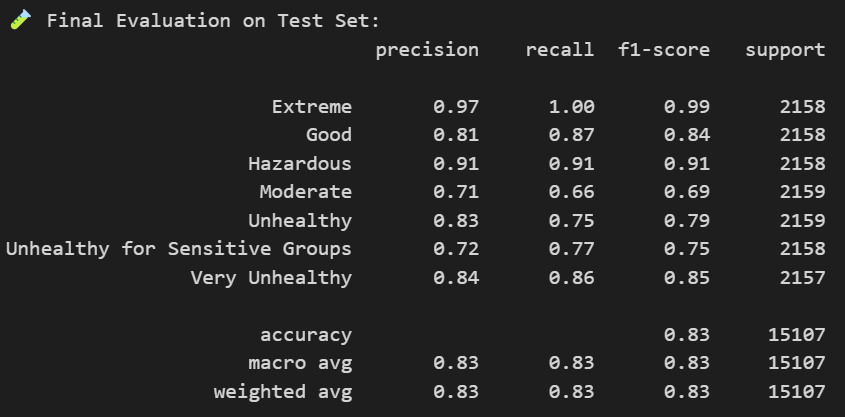
\includegraphics[width=0.7\linewidth]{41}
	\caption{گزارش طبقه بندی مدل DE}
	\label{fig:41}
\end{figure}

\begin{figure}[h!]
	\centering
	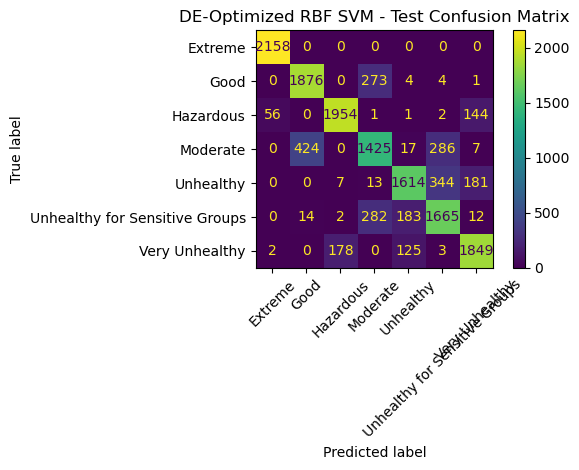
\includegraphics[width=0.7\linewidth]{42}
	\caption{ماتریس در هم ریختگی مدل DE}
	\label{fig:42}
\end{figure}

\begin{figure}[h!]
	\centering
	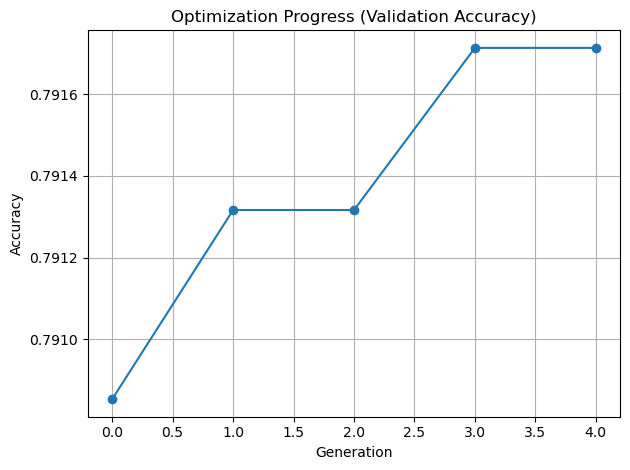
\includegraphics[width=0.7\linewidth]{43}
	\caption{فرایند بهینه سازی مدل با DE}
	\label{fig:43}
\end{figure}



سپس ارزیابی روی مجموعه‌ی تست صورت گرفت و گزارش کامل طبقه‌بندی و ماتریس درهم‌ریختگی (\lr{Confusion Matrix}) ترسیم گردید.

در نهایت، نموداری رسم شده که روند پیشرفت دقت الگوریتم \lr{DE} را در طی نسل‌ها نشان می‌دهد.

\vspace{1em}

این روش نه‌تنها باعث بهینه‌سازی خودکار پارامترهای حساس مدل \lr{SVM} شد، بلکه بدون نیاز به جستجوی دستی یا تنظیمات تجربی، مدلی دقیق و پایدار تولید کرد. همچنین مشاهده شد که حتی با تعداد کمی نسل، الگوریتم \lr{DE} توانست به دقت قابل قبولی دست یابد.
\subsubsection{1.3.6}

به‌منظور آماده‌سازی داده‌های ورودی برای مدل یادگیری ماشین، مجموعه‌ای از مراحل پیش‌پردازش و مهندسی ویژگی بر روی داده‌ها اعمال گردید. این مراحل به‌گونه‌ای طراحی شده‌اند که هم ویژگی‌های مفیدی از تاریخچه آلودگی استخراج شود، و هم داده‌ها از نظر کیفی برای تغذیه به مدل \lr{SVM} آماده گردند. مراحل به شرح زیر بوده‌اند:

\begin{enumerate}
	\item \textbf{حذف ستون‌های اضافی:} ستون \lr{No} که صرفاً شماره ردیف بود، حذف گردید.
	\item \textbf{ایجاد ویژگی‌های تاخیری:} برای متغیر \lr{pm2.5}، مقادیر مربوط به ۱، ۲، ۳، ۲۴ و ۱۶۸ ساعت قبل به‌عنوان ویژگی جدید ایجاد شد.
	\item \textbf{حذف مقادیر گمشده:} ردیف‌هایی که در هر یک از ویژگی‌های اصلی یا تاخیری مقدار \lr{NaN} داشتند، حذف شدند.
	\item \textbf{کدگذاری جهت باد:} ستون \lr{cbwd} به‌صورت \lr{One-Hot} کدگذاری شد.
	\item \textbf{مدیریت داده‌های پرت:} ستون \lr{Iws} که مربوط به سرعت تجمعی باد است، در بازه صدک اول و نود و نهم بریده شد (capping).
	\item \textbf{استخراج ویژگی‌های آماری ساعتی:} برای متغیر \lr{pm2.5}، با استفاده از پنجره‌ای ۲۴ ساعته، ویژگی‌هایی مانند میانگین، انحراف معیار، واریانس، کمینه، بیشینه، میانه، چولگی و کشیدگی استخراج گردید.
	\item \textbf{طبقه‌بندی آلودگی:} با استفاده از مقدار \lr{pm2.5}، ردیف‌ها به دسته‌های استاندارد کیفیت هوا طبقه‌بندی شدند (\lr{AQI Category}).
	\item \textbf{کدگذاری برچسب هدف:} دسته‌بندی کیفی با استفاده از \lr{LabelEncoder} به مقدار عددی تبدیل شد تا برای مدل قابل استفاده باشد.
	\item \textbf{ویژگی‌های چرخه‌ای:} مقادیر \lr{hour}، \lr{month} و \lr{weekday} با استفاده از تبدیل‌های سینوسی و کسینوسی به ویژگی‌هایی چرخه‌ای تبدیل شدند.
	\item \textbf{کدگذاری فصل‌ها:} ماه‌ها به فصل‌های سال نگاشت شدند و با استفاده از توابع سینوس و کسینوس برای الگوهای دوره‌ای کدگذاری شدند.
	\item \textbf{استخراج رکورد نهایی برای پیش‌بینی:} پس از انجام تمامی مراحل، آخرین ردیف (که هنوز مقدار هدف آن مشخص نیست) به‌عنوان ورودی به مدل پیش‌بینی داده شد، در حالی که فقط از ۱۰ ویژگی مهم استفاده شده است.
\end{enumerate}

این فرایند باعث افزایش کیفیت و پایداری مدل و همچنین استخراج ویژگی‌های وابسته به زمان شد که در پیش‌بینی آلودگی بسیار مؤثر هستند.













\newpage

\section{کاهش ابعاد}

برای مشاهده نوت‌بوک من اینجا کلیک کنید: \href{https://colab.research.google.com/drive/19FeKvQRYjtjR0_xEpMn-Ow_VjjoD6UuD?usp=sharing}{لینک گوگل کولب}

\subsection{سوالات}

\subsubsection{الف}

کد پایتون این بخش برای بارگذاری و پردازش مجموعه داده \lr{Fashion MNIST} طراحی شده است که شامل ۷۰,۰۰۰ تصویر سیاه‌وسفید ۲۸×۲۸ پیکسل از ۱۰ دسته مختلف پوشاک است. ابتدا داده‌های آموزشی از این مجموعه بارگذاری می‌شوند و از هر دسته (مانند تی‌شرت، شلوار و غیره) یک تصویر به‌صورت تصادفی انتخاب می‌شود. سپس این تصاویر در یک ردیف نمایش داده می‌شوند.\autoref{f211} در ادامه، نویز گاوسی با میانگین صفر و انحراف معیار ۰٫۲ به تصاویر اضافه می‌شود تا نسخه‌های نویزی آن‌ها ایجاد شود. مقادیر پیکسل‌ها به بازه [0, 1] نرمال‌سازی و محدود می‌شوند. در نهایت، تصاویر نویزی نیز در یک ردیف جداگانه نمایش داده می‌شوند \autoref{f212} تا امکان مقایسه با تصاویر اصلی فراهم شود \autoref{f213}.


\begin{figure}[h!]
    \centering
    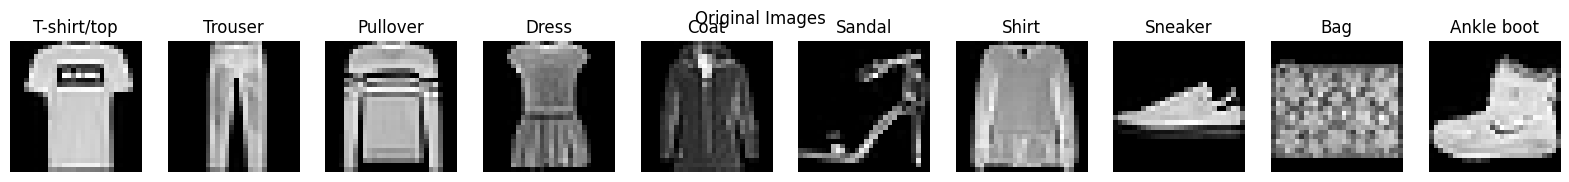
\includegraphics[width=1\linewidth]{Q21_1.png}
    \caption{تصاویر اصلی}
    \label{f211}
\end{figure}


\begin{figure}[h!]
    \centering
    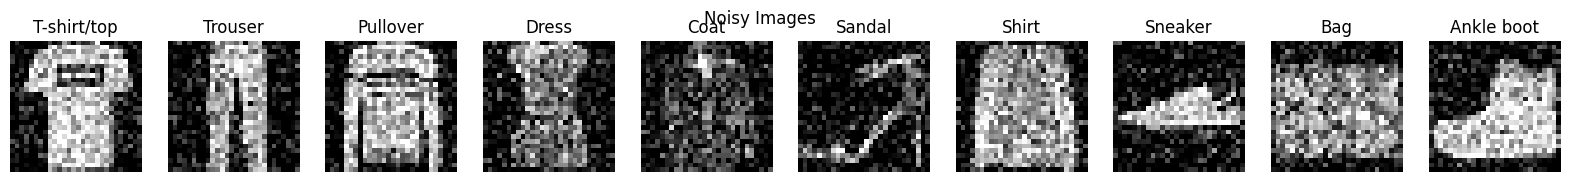
\includegraphics[width=1\linewidth]{Q21_2.png}
    \caption{تصاویر نویزی}
    \label{f212}
\end{figure}


\begin{figure}[h!]
    \centering
    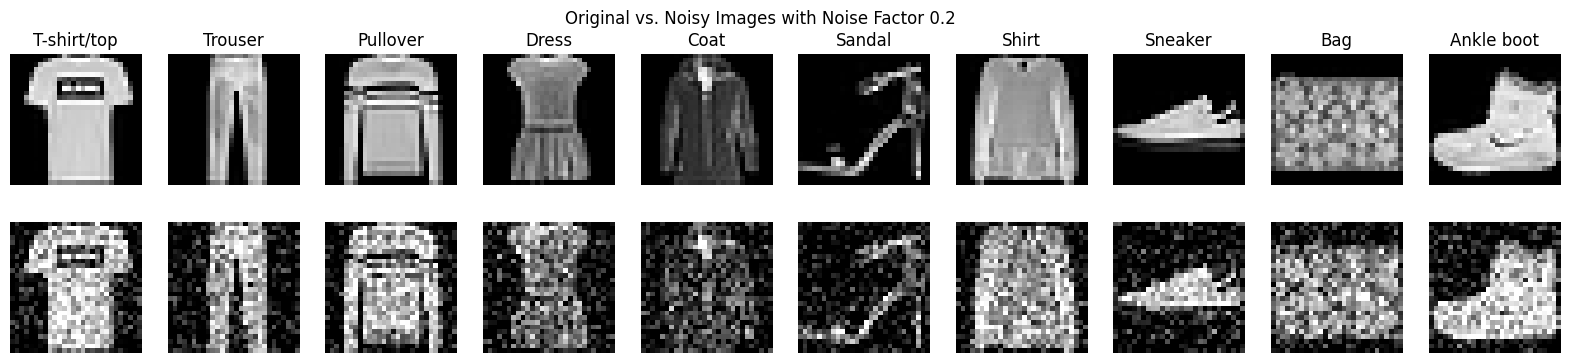
\includegraphics[width=1\linewidth]{Q21_3.png}
    \caption{تصاویر اصلی و نویزی در کنار هم}
    \label{f213}
\end{figure}


\subsubsection{ب}

این بخش کد پایتون الگوریتم تحلیل مؤلفه‌های اصلی \lr{(PCA)} را بدون استفاده از کتابخانه‌های آماده برای مجموعه داده \lr{Fashion MNIST} پیاده‌سازی می‌کند. ابتدا تصاویر ۲۸×۲۸ پیکسل به بردارهای ۷۸۴ بعدی تبدیل شده و داده‌ها نرمال‌سازی و استانداردسازی می‌شوند. سپس ماتریس کوواریانس داده‌ها محاسبه شده و مقادیر ویژه و بردارهای ویژه آن به ترتیب نزولی مرتب می‌شوند. نسبت واریانس توضیح‌داده‌شده برای هر مؤلفه اصلی و واریانس تجمعی محاسبه می‌شود تا مشخص شود چند مؤلفه برای حفظ حداقل ۹۰٪ از واریانس کل کافی است. در نهایت، نتایج به‌صورت یک نمودار میله‌ای و خطی ( \autoref{f221} و \autoref{f223} ) نمایش داده می‌شود که نسبت واریانس توضیح‌داده‌شده و واریانس تجمعی را نشان می‌دهد.

\begin{figure}[h!]
    \centering
    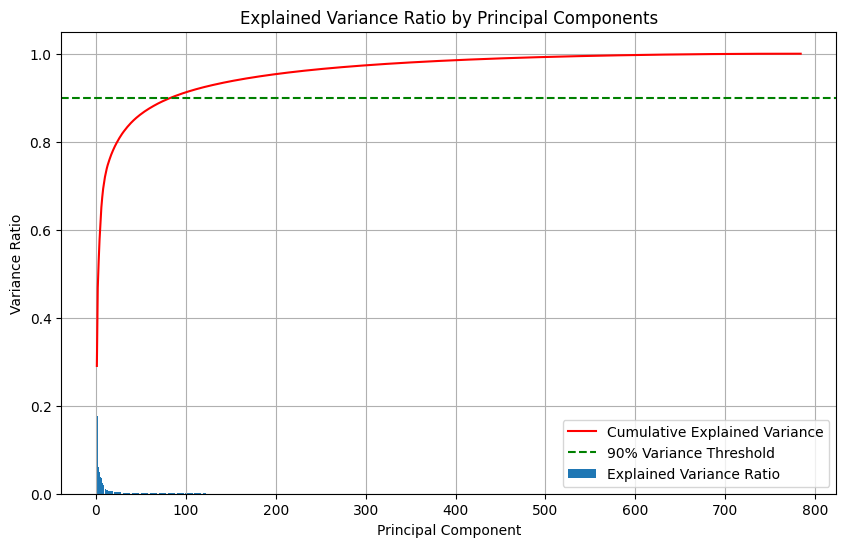
\includegraphics[width=1\linewidth]{Q22_1.png}
    \caption{نمودار واریانس تجمعی بر اساس مولفه ها}
    \label{f221}
\end{figure}


\begin{figure}[h!]
    \centering
    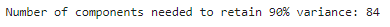
\includegraphics[width=1\linewidth]{Q22_2.png}
    \caption{مشاهده خروجی کد یعنی تعداد مولفه های اصلی کافی}
    \label{f222}
\end{figure}


\begin{figure}[h!]
    \centering
    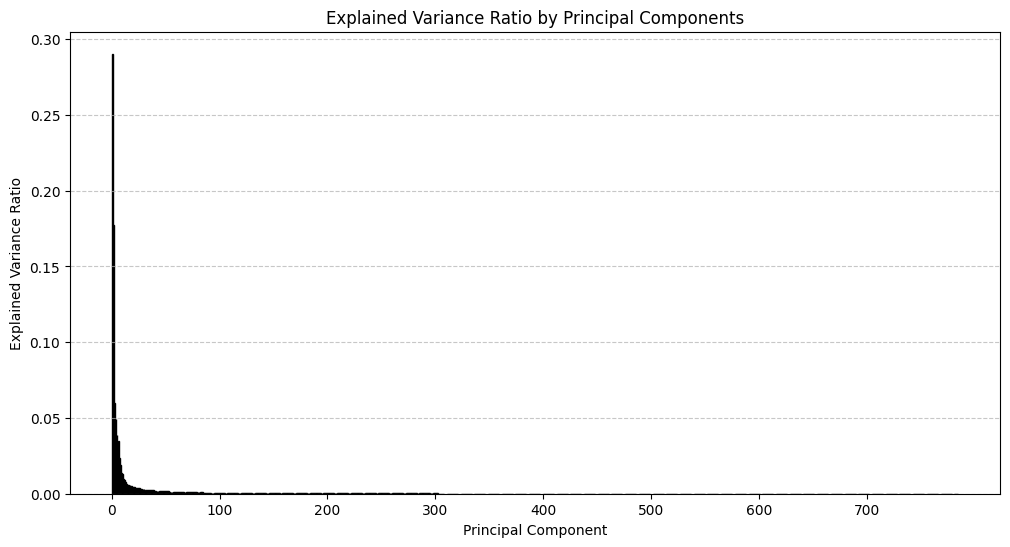
\includegraphics[width=1\linewidth]{Q22_3.png}
    \caption{نمودار میله ای واریانس تجمعی بر اساس مولفه ها}
    \label{f223}
\end{figure}


خروجی این کد شامل یک نمودار و یک مقدار عددی (\autoref{f222}) است. نمودار با عنوان \lr{"Explained Variance Ratio by Principal Components"} یک خط قرمز برای واریانس تجمعی و یک خط افقی سبز در سطح ۹۰٪ واریانس را نمایش می‌دهد. خط قرمز نشان می‌دهد که واریانس تجمعی با افزایش تعداد مؤلفه‌ها به‌سرعت رشد می‌کند و در حدود مؤلفه ۸۴ به آستانه ۹۰٪ می‌رسد. همچنین، خروجی عددی کد نشان می‌دهد که برای حفظ ۹۰٪ از واریانس کل داده‌ها، به ۸۴ مؤلفه اصلی نیاز است، که این تعداد مؤلفه بخش عمده اطلاعات داده را حفظ می‌کند و برای کاهش ابعاد داده مناسب است.

\subsubsection{ج}

این بخش کد پایتون با استفاده از کتابخانه \lr{`scikit-learn`} الگوریتم تحلیل مؤلفه‌های اصلی \lr{(PCA)} را بر روی مجموعه داده \lr{(PCA)} اعمال می‌کند تا ابعاد داده‌ها را کاهش دهد. ابتدا تصاویر ۲۸×۲۸ پیکسلی این مجموعه که شامل ۷۰,۰۰۰ تصویر از ۱۰ دسته مختلف پوشاک است، به بردارهای ۷۸۴ بعدی تبدیل شده و مقادیر پیکسل‌ها به بازه [0, 1] نرمال‌سازی می‌شوند. سپس PCA با تنظیم دو مؤلفه اصلی اجرا می‌شود تا داده‌ها به یک فضای دوبعدی کاهش یابند. در نهایت، یک نمودار پراکندگی دوبعدی رسم می‌شود (\autoref{f231}) که هر دسته با رنگی متفاوت نشان داده می‌شود، به‌منظور تحلیل بصری توزیع داده‌ها و جداسازی دسته‌ها پس از کاهش ابعاد. در این نمودار، هر نقطه نشان‌دهنده یک تصویر است و نقاط مربوط به هر یک از ۱۰ دسته (مانند تی‌شرت، شلوار، کفش و غیره) با رنگ‌های متمایز مشخص شده‌اند. محورهای x و y به‌ترتیب مؤلفه‌های اصلی اول و دوم را نشان می‌دهند. با وجود اینکه ممکن است برخی دسته‌ها به دلیل پیچیدگی داده‌ها هم‌پوشانی داشته باشند، الگوهای کلی توزیع دسته‌ها قابل مشاهده است، که این امر به درک بهتر ساختار داده‌ها پس از کاهش ابعاد کمک می‌کند.


\begin{figure}[h!]
    \centering
    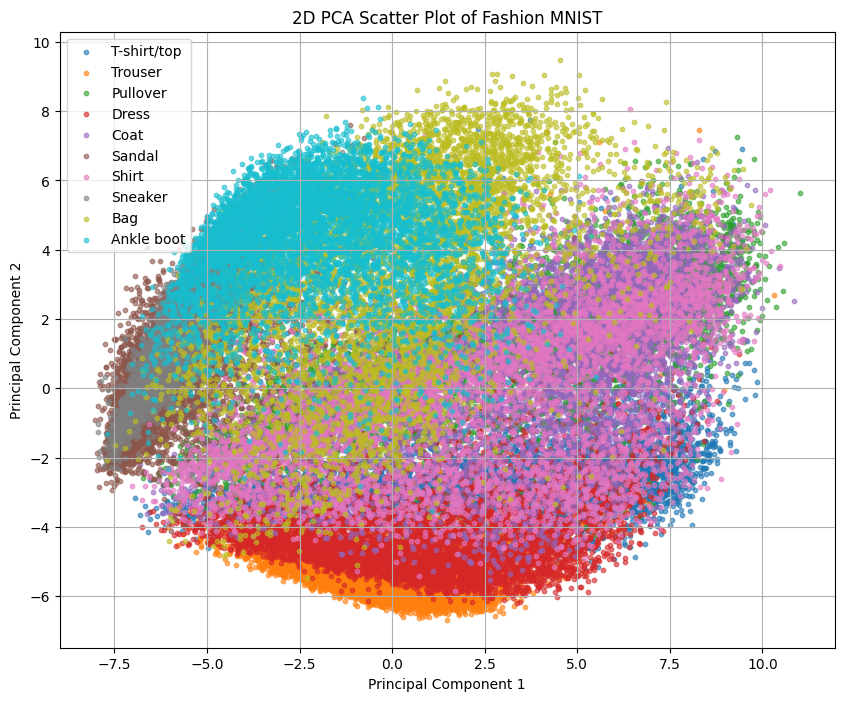
\includegraphics[width=1\linewidth]{Q23_1.png}
    \caption{نمودار PCA}
    \label{f231}
\end{figure}

\newpage

\subsubsection{د}

خروجی کد این بخش شامل یک نمودار سه‌ردیفه است که شامل ۱۰ تصویر از هر دسته \lr{Fashion MNIST} است(\autoref{f241}). ردیف اول تصاویر اصلی را نشان می‌دهد که واضح و بدون نویز هستند. ردیف دوم تصاویر نویزی را نمایش می‌دهد که به دلیل افزودن نویز گاوسی، کیفیت آن‌ها کاهش یافته و دانه‌دار به نظر می‌رسند. ردیف سوم تصاویر بازسازی‌شده با استفاده از ۱۰۰ مؤلفه اصلی PCA را نشان می‌دهد که نسبت به نسخه نویزی واضح‌تر هستند، اما برخی جزئیات ریز به دلیل کاهش ابعاد از دست رفته و تصاویر کمی تار به نظر می‌رسند. این مقایسه نشان‌دهنده توانایی PCA در حذف نویز با حفظ ساختار کلی تصاویر است. در ادامه و در \autoref{f242} ما با 500 مولفه اصلی سعی کردیم که تصاویر نویزی را بازسازی کنیم که تا حدودی موفق شدیم و به نتیجه مطلوب تری نسبت به 100 مولفه رسیدیم.


\begin{figure}[h!]
    \centering
    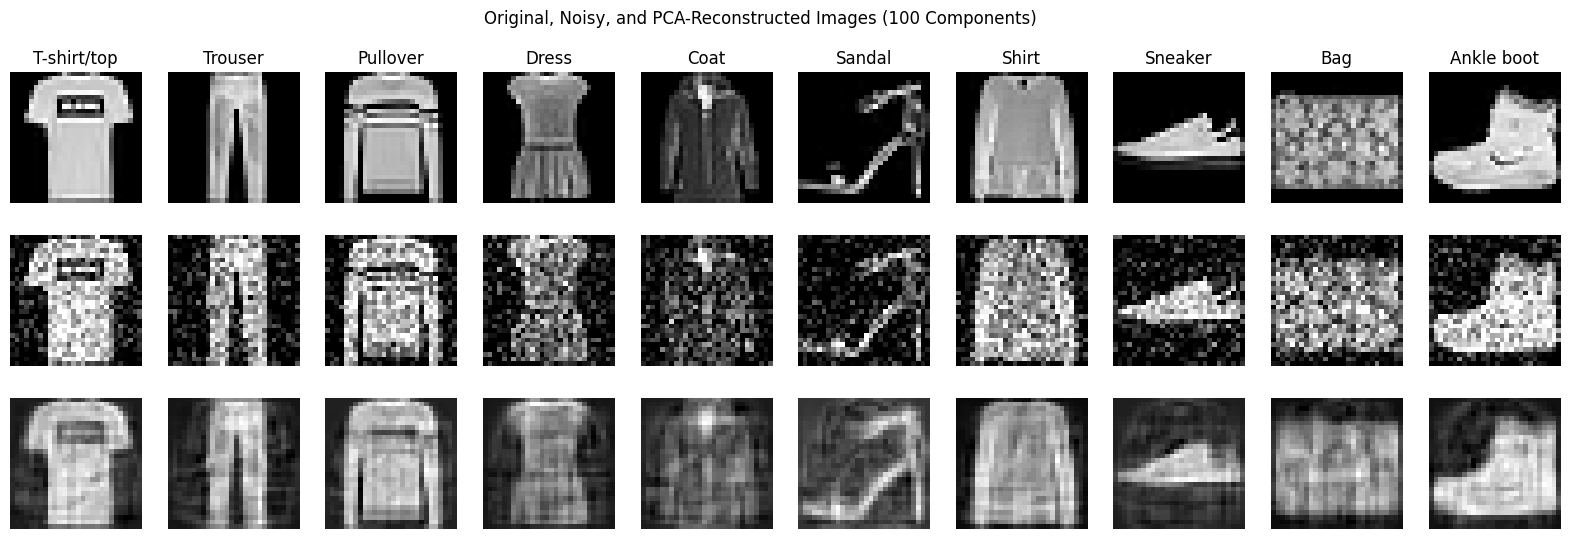
\includegraphics[width=1\linewidth]{Q24_1.png}
    \caption{تصاویر اصلی و نویزی و بازسازی شده در کنار هم با 100 مولفه اصلی}
    \label{f241}
\end{figure}


\begin{figure}[h!]
    \centering
    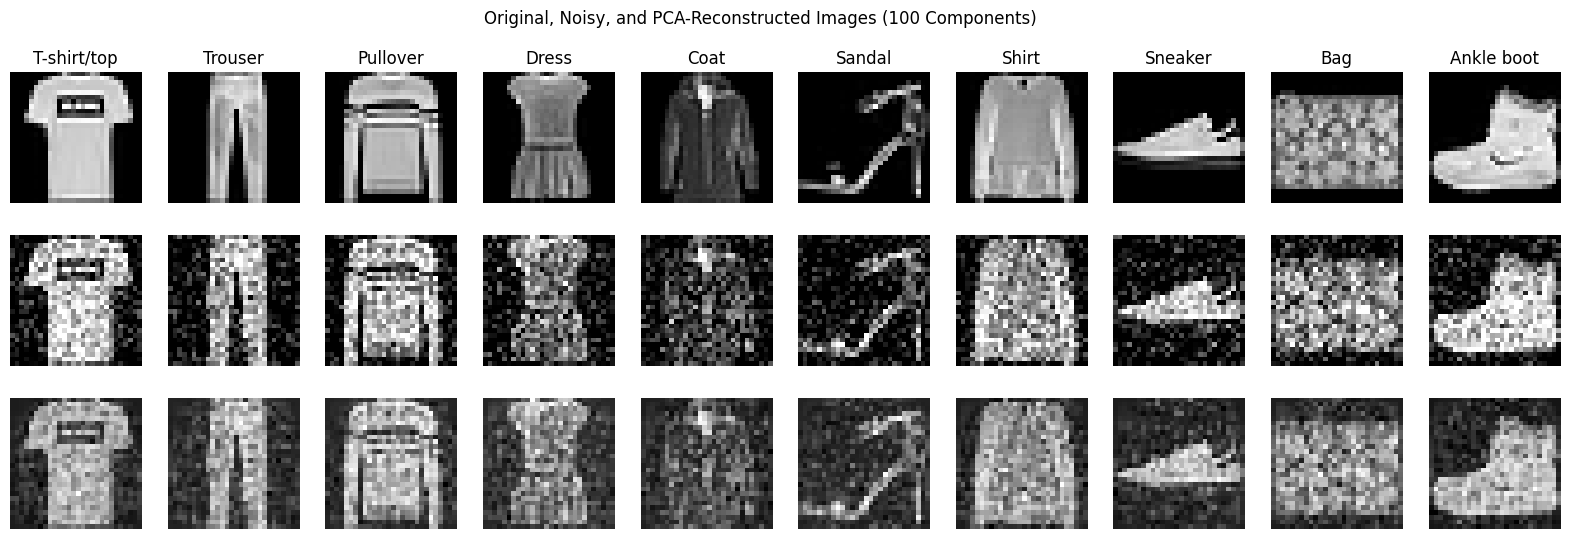
\includegraphics[width=1\linewidth]{Q24_2.png}
    \caption{تصاویر اصلی و نویزی و بازسازی شده در کنار هم با 500 مولفه اصلی}
    \label{f242}
\end{figure}


\subsubsection{ه}

این کد پایتون الگوریتم تحلیل تمایزی خطی (LDA) را با استفاده از کتابخانه \lr{`scikit-learn`} بر روی مجموعه داده \lr{Fashion MNIST} پیاده‌سازی می‌کند تا ابعاد داده‌ها را کاهش دهد. ابتدا تصاویر ۲۸×۲۸ پیکسلی این مجموعه که شامل ۷۰,۰۰۰ تصویر از ۱۰ دسته مختلف پوشاک است، به بردارهای ۷۸۴ بعدی تبدیل شده و مقادیر پیکسل‌ها به بازه [0, 1] نرمال‌سازی می‌شوند. سپس LDA با تنظیم دو مؤلفه اجرا می‌شود تا داده‌ها به یک فضای دوبعدی کاهش یابند، با این هدف که جداسازی بین کلاس‌ها حداکثر شود. در نهایت، یک نمودار پراکندگی دوبعدی رسم می‌شود(\autoref{f251}) که هر دسته با رنگی متفاوت نمایش داده می‌شود و نسبت واریانس توضیح‌داده‌شده توسط مؤلفه‌های LDA محاسبه و چاپ می‌شود(\autoref{f252}). جداسازی بین دسته‌ها نسبت به PCA واضح‌تر است، زیرا LDA بر تمایز بین کلاس‌ها تمرکز دارد. همچنین، نسبت واریانس توضیح‌داده‌شده توسط مؤلفه‌های LDA برابر با [0.6543, 0.3457] است، که نشان می‌دهد مؤلفه اول ۶۵٫۴۳٪ و مؤلفه دوم ۳۴٫۵۷٪ از واریانس داده‌های تبدیل‌شده را توضیح می‌دهند، و مجموع آن‌ها ۱۰۰٪ است، زیرا فقط دو مؤلفه در نظر گرفته شده است.


\begin{figure}[h!]
    \centering
    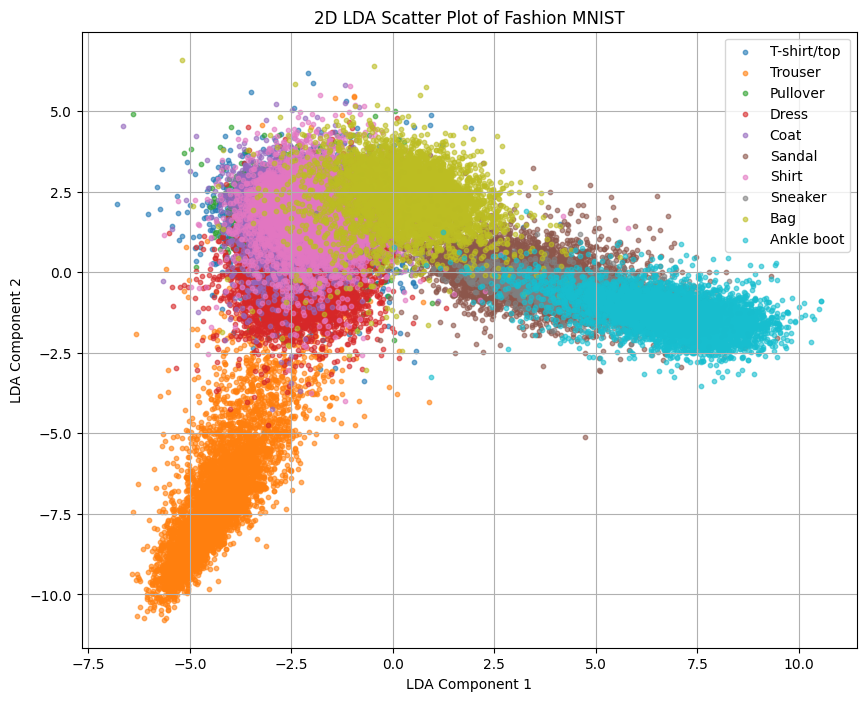
\includegraphics[width=1\linewidth]{Q25_1.png}
    \caption{نمودار LDA}
    \label{f251}
\end{figure}


\begin{figure}[h!]
    \centering
    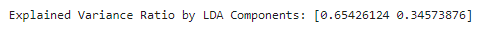
\includegraphics[width=1\linewidth]{Q25_2.png}
    \caption{نسبت واریانس مولفه اول و مولفه دوم}
    \label{f252}
\end{figure}


\subsubsection{و}

این بخش به‌منظور محاسبه و تحلیل ماتریس‌های پراکندگی درون‌کلاسی (Sw) و بین‌کلاسی (Sb) در چارچوب الگوریتم تحلیل تمایزی خطی (LDA) برای مجموعه داده \lr{Fashion MNIST} طراحی شده است. ابتدا تصاویر ۲۸×۲۸ پیکسلی این مجموعه به بردارهای ۷۸۴ بعدی تبدیل و نرمال‌سازی می‌شوند، و یک زیرمجموعه ۲۰۰۰ تایی از داده‌ها برای کارایی محاسباتی انتخاب می‌شود. ماتریس Sw با جمع پراکندگی درون هر کلاس و ماتریس Sb با استفاده از تفاوت میانگین کلاس‌ها از میانگین کلی محاسبه می‌شود. سپس، ماتریس جدایی‌پذیری \lr{\( (S^{-1}_w \cdot S_b) \)} با اعمال یک هموارسازی کوچک برای جلوگیری از تکین بودن Sw تشکیل شده، و مقادیر ویژه این ماتریس به‌صورت نزولی محاسبه و در یک نمودار میله‌ای نمایش داده می‌شود (\autoref{f261}). نمودار نشان می‌دهد که چند مقدار ویژه اول (مانند ۳۹۷٫۸۴ و ۱۳۹٫۴۱) به‌طور قابل‌توجهی بزرگ‌تر از بقیه هستند، در حالی که مقادیر بعدی به‌سرعت به صفر یا مقادیر منفی نزدیک می‌شوند، که این امر بیانگر وجود چند جهت اصلی برای تمایز بین کلاس‌ها است. پنج مقدار ویژه برتر به ترتیب ۳۹۷٫۸۴، ۱۳۹٫۴۱، ۱۰۷٫۳۸، ۸۲٫۳۹ و ۷۳٫۸۰ گزارش شده‌اند، که نشان می‌دهد مؤلفه‌های اولیه بیشترین اطلاعات جداسازی را حمل می‌کنند و استفاده از تعداد محدودی از این مؤلفه‌ها می‌تواند برای کاهش ابعاد کافی باشد.


\begin{figure}[h!]
    \centering
    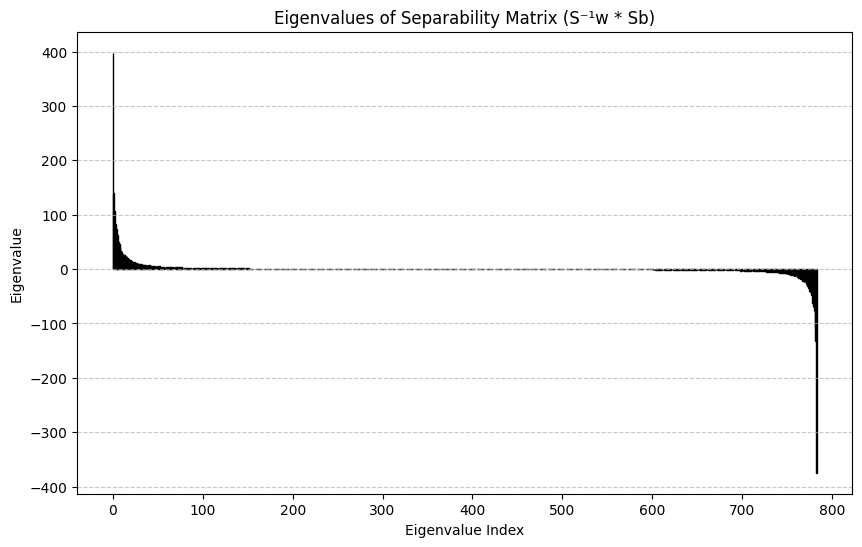
\includegraphics[width=1\linewidth]{Q26_1.png}
    \caption{نمودار میله ای مقادیر ویژه}
    \label{f261}
\end{figure}


\begin{figure}[h!]
    \centering
    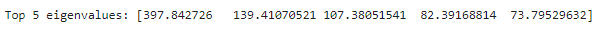
\includegraphics[width=1\linewidth]{Q26_2.png}
    \caption{5 مقدار ویژه برتر}
    \label{f262}
\end{figure}


\subsubsection{ز}

این بخش به‌منظور بررسی تأثیر تعداد ویژگی‌ها بر مقدار ردیابی ماتریس جدایی‌پذیری \lr{\( (S^{-1}_w \cdot S_b) \)} در چارچوب تحلیل تمایزی خطی (LDA) برای مجموعه داده \lr{Fashion MNIST} طراحی شده است. ابتدا تصاویر ۲۸×۲۸ پیکسلی این مجموعه به بردارهای ۷۸۴ بعدی تبدیل و نرمال‌سازی شده، و یک زیرمجموعه ۲۰۰۰ تایی از داده‌ها برای محاسبات انتخاب می‌شود. ماتریس‌های پراکندگی درون‌کلاسی (Sw) و بین‌کلاسی (Sb) برای تعداد مختلف ویژگی‌ها (از ۵۰ تا ۷۸۴ با گام ۵۰) محاسبه می‌شوند، و با اعمال یک هموارسازی کوچک برای جلوگیری از تکین بودن Sw، ماتریس جدایی‌پذیری تشکیل و مقدار ردیابی آن محاسبه می‌شود. در نهایت، این مقادیر در یک نمودار خطی رسم شده (\autoref{f271}) و تعداد بهینه ویژگی‌ها بر اساس حداکثر ردیابی تعیین می‌شود (\autoref{f272}). نمودار نشان می‌دهد که با افزایش تعداد ویژگی‌ها از ۵۰ به ۷۵۰، مقدار ردیابی به‌صورت مداوم از حدود ۵ به بیش از ۵۰ افزایش می‌یابد، که بیانگر بهبود جداسازی کلاس‌ها با افزودن ویژگی‌های بیشتر است. با این حال، تعداد بهینه ویژگی‌ها ۷۵۰ گزارش شده است، که نشان می‌دهد پس از این نقطه، افزودن ویژگی‌های بیشتر تأثیر قابل‌توجهی بر ردیابی ندارد و ممکن است نویز اضافه کند. این نتیجه نشان‌دهنده تعادل بهینه بین اطلاعات جداسازی و پیچیدگی مدل است.


\begin{figure}[h!]
    \centering
    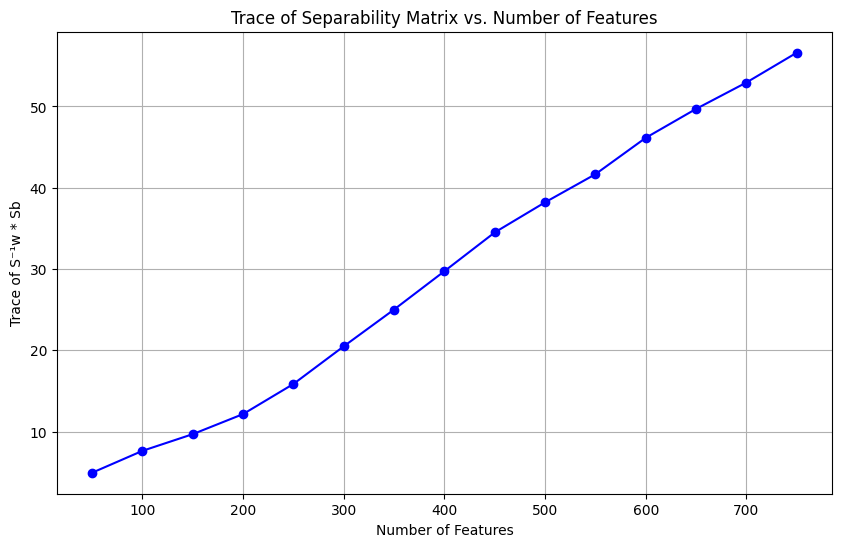
\includegraphics[width=1\linewidth]{Q27_1.png}
    \caption{نمودار خطی trace}
    \label{f271}
\end{figure}


\begin{figure}[h!]
    \centering
    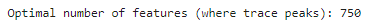
\includegraphics[width=1\linewidth]{Q27_2.png}
    \caption{ مقدار بهینه ویژگی ها}
    \label{f272}
\end{figure}


\subsection{امتیازی}

\lr{t-SNE (t-distributed Stochastic Neighbor Embedding)} یک روش کاهش ابعاد غیرخطی است که برای تجسم داده‌های با ابعاد بالا در فضاهای دو یا سه‌بعدی طراحی شده است. این روش ابتدا فاصله‌های بین نقاط داده در فضای اصلی را با استفاده از توزیع‌های گاوسی به احتمالات شباهت تبدیل می‌کند، به‌طوری‌که نقاط نزدیک‌تر احتمال شباهت بیشتری دارند. سپس، در فضای کاهش‌یافته (مثلاً دوبعدی)، از توزیع t-student برای مدل‌سازی شباهت‌ها استفاده می‌کند و تلاش می‌کند با کمینه کردن اختلاف \lr{(Divergence Kullback-Leibler)} بین این دو توزیع، ساختار محلی داده‌ها را حفظ کند. t-SNE بیشتر برای تجسم داده‌ها مناسب است و بر حفظ ساختارهای محلی (مانند خوشه‌ها) تمرکز دارد، اما ممکن است ساختارهای جهانی را به‌خوبی حفظ نکند.

این بخش الگوریتم \lr{t-SNE (t-distributed Stochastic Neighbor Embedding)} را بدون استفاده از کتابخانه‌های آماده برای کاهش ابعاد داده‌های مجموعه \lr{Fashion MNIST} پیاده‌سازی می‌کند. ابتدا تصاویر ۲۸×۲۸ پیکسلی این مجموعه به بردارهای ۷۸۴ بعدی تبدیل و نرمال‌سازی شده، و یک زیرمجموعه ۱۰۰۰ تایی از داده‌ها برای کارایی محاسباتی انتخاب می‌شود. الگوریتم با محاسبه فاصله‌های اقلیدسی در فضای اصلی و تبدیل آن‌ها به احتمالات با توزیع گاوسی (Pij) آغاز می‌شود، سپس در فضای کاهش‌یافته با استفاده از توزیع \lr{t-student (Qij)} شباهت‌ها را مدل می‌کند. با استفاده از گرادیان نزولی و کمینه کردن اختلاف \lr{Kullback-Leibler}، داده‌ها به دو بعد کاهش یافته و در یک نمودار پراکندگی با رنگ‌های متفاوت برای هر کلاس نمایش داده می‌شوند (\autoref{f281}). در این نمودار، هر نقطه نماینده یک تصویر است و نقاط مربوط به ۱۰ دسته (مانند تی‌شرت، شلوار و غیره) با رنگ‌های متمایز مشخص شده‌اند. خوشه‌بندی محلی قابل‌توجهی در این نمودار مشاهده می‌شود، به‌طوری‌که دسته‌هایی مانند شلوار و کفش به‌خوبی از هم جدا شده‌اند، اما فواصل جهانی ممکن است تحریف شده باشند. این نتیجه نشان‌دهنده توانایی t-SNE در حفظ ساختارهای محلی و تجسم داده‌های پیچیده است، هرچند مقیاس محورها بسیار کوچک (در حد ۰٫۰۰۰۰x) است که به دلیل حساسیت الگوریتم به پارامترها و نرخ یادگیری است.


\begin{figure}[h!]
    \centering
    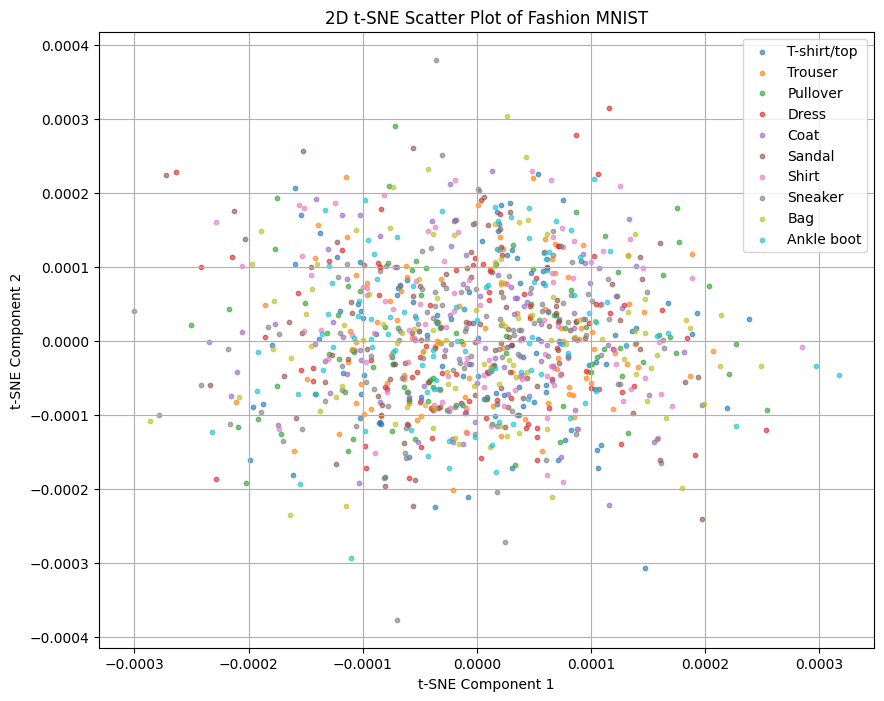
\includegraphics[width=1\linewidth]{Q28_1.png}
    \caption{نمودار t-SNE}
    \label{f281}
\end{figure}

\textcolor{red}{مقایسه با PCA و LDA:}

\textcolor{blue}{مزایای t-SNE:}

حفظ ساختار محلی: t-SNE در تجسم خوشه‌های محلی و جداسازی داده‌های پیچیده بسیار قوی است، و اغلب خوشه‌های واضح‌تری نسبت به PCA و LDA ایجاد می‌کند.

غیرخطی بودن: بر خلاف PCA و LDA که روش‌های خطی هستند، t-SNE می‌تواند روابط غیرخطی را مدل کند، که برای داده‌های پیچیده مانند \lr{Fashion MNIST} مفید است.

\textcolor{blue}{محدودیت‌های t-SNE:}

عدم حفظ ساختار جهانی: t-SNE بر ساختار محلی تمرکز دارد و ممکن است فواصل جهانی بین خوشه‌ها را تحریف کند، در حالی که PCA ساختار جهانی را بهتر حفظ می‌کند.

پیچیدگی محاسباتی: t-SNE محاسبات سنگین‌تری دارد \( O(n^2) \) و برای داده‌های بزرگ کند است، در حالی که PCA و LDA سریع‌تر هستند.

حساسیت به پارامترها: t-SNE به تنظیمات perplexity و نرخ یادگیری حساس است، که می‌تواند نتایج را تغییر دهد.

عدم قطعیت: t-SNE یک روش احتمالی است و نتایج ممکن است در هر اجرا متفاوت باشند، در حالی که PCA و LDA قطعی هستند.

\textcolor{red}{مقایسه با PCA و LDA:}

PCA (بخش ج): PCA واریانس کل را حداکثر می‌کند و ساختار جهانی را حفظ می‌کند، اما جداسازی کلاس‌ها ضعیف‌تر است (هم‌پوشانی زیاد در نمودار پراکندگی).

LDA (بخش ه): LDA بر جداسازی کلاس‌ها تمرکز دارد و به دلیل نظارت‌شده بودن، جداسازی بهتری نسبت به PCA ارائه می‌دهد، اما همچنان خطی است و ممکن است برای داده‌های غیرخطی مثل \lr{Fashion MNIST} کافی نباشد.

\lr{t-SNE}: در تجسم خوشه‌های محلی و جداسازی غیرخطی بهتر عمل می‌کند، اما برای وظایف کاهش ابعاد عمومی (مثلاً پیش‌پردازش برای یادگیری ماشین) مناسب نیست، در حالی که PCA و LDA کاربردهای گسترده‌تری دارند.




\end{document}